\section{Evoluzione stellare}\linkdest{stellarevolution}

\begin{wordonframe}{da fare: kippenhahn wiegert}
\begin{itemize}
\item main sequence 207'-214' (110-114)
\item Hayashi line 224'-232' (119-123)
\item Stability 234'-246 (124-130)
\item Onset of star formation 248'-255' (131-134)
\item Formation of protostars 256'-265' (135-139)
\item pre-main sequence contraction 266'-270' (140-142)
\item from initial to present sun 271'-276' (142-144)
\item chemical evolution in MS 277'-291' (145-152)
\item He-burning: massive stars 292'-307' (153-160)
\item He-burning:low-mass stars 308'-327' (161-170)
\item Later phases:  328'-343' (171-178)
\item Explosion and collapse 344'-364' (179-189)
\end{itemize}
\end{wordonframe}

\begin{frame}[allowframebreaks]{List of things}
%\printbibliography[keyword={inference},heading=beamer]
%\printbibliography[keyword={\mybibcat},heading=beamer]
\listofkeywords
\end{frame}

\subsection{Pre main sequence ed approccio a ZAMS per stelle di sequenza superiori/inferiori}\linkdest{preMS}

\begin{frame}{Traccia di Hayashi}
Primo/secondo core di Larson; Evoluzione di PMS sulla traccia di Hayashi; ruolo di opacit\'a di H- nella verticalit\'a della traccia di Hayashi; fusione deuterio; stelle completamente convettive o con nucleo radiativo. Abbondanza elementi leggeri in stelle di pre-sequenza
\end{frame}

\begin{frame}{Approccio alla ZAMS per stelle di sequenza superiori/inferiori}
dipendenza della ZAMS dall'abbondanza originale di He e metalli; metodo determinazione $DY/DZ$ dal confronto teoria-osservazione per stelle di disco locale parallassate; dipendenza massa minima di transizione dall'abbondanza di He e metalli; influenza sulla ZAMS dell'incertezza degli input fisici e dell'efficienza della convezione
\end{frame}

\subsection{Evoluzione di sequenza principale}\linkdest{MS}

\begin{frame}{Yield of H-burning star analysis}
\begin{itemize}
\item Longest evolutionary phase: larger number of observed stars
\item central/shell-H-burning determine successive phases
\item most important clock is central H-burning termination
\item Final shell H-burning phase in low mass, low-Z star provide distance indicator for old stellar pop
\item count of stars evolving through central H-burning give insight on IMF
\end{itemize}
\end{frame}

\begin{frame}{Major H burning reaction: PP chains}
\begin{columns}[T]\begin{column}{0.45\textwidth}
\begin{align*}
&T\leq\SI{5e6}{\kelvin}\\
&^1H+^1H\to^2D+\APelectron+\Pnue\\
&^2D+^1H\to^3He+\gamma\\
&T\geq\SI{8e6}{\kelvin}:\\
&^3He+^3He\to^4He+2^1H\tag*{PPI}\\
&T\geq\SI{15e6}{\kelvin}:\\
&^3He+^4He\to^7Be+\gamma\\
&^7Be+\Pelectron\to^7Li+\Pnue\\
&^7Li+^1H\to^4He+^4He\tag*{PPII}\\
&^7Be+^1H\to^8B+\gamma\\
&^8B\to^8Be+\APelectron+\gamma\\
&^8Be\to2^4He
\end{align*}
\end{column}\begin{column}{0.55\textwidth}
\begin{align*}
&r_{pp}=\num{11.5e10}\rho^2X_H^2T_6\expy{-2/3}\\
&\exp{-33.81T_6\expy{-1/3}}(1+\num{0.0123}T_6\expy{1/3}+\num{0.0109}T_6\expy{2/3}\\
&+\num{0.00095}T_6)\\
&\rho\epsilon(3H\to^3He)=\\
&(\SI{6.936}{\mega\ev}-\SI{0.263}{\mega\ev})*\SI{1.602e-6}{\erg}*r_{pp}\\
&\rho\epsilon(^3He(^3He,2p)^4He)=\\
&(\SI{6.936}{\mega\ev}-\SI{0.263}{\mega\ev})*\SI{1.602e-6}{\erg}*r_{pp}\\
&\frac{PPI}{PPII+PPIII}=\frac{r_{33}}{r_{34}}=\frac{\lambda_{33}(^3He)^2/2}{\lambda_{34}^3He^4He}
\end{align*}
\end{column}\end{columns}
\end{frame}

\begin{frame}{H burning: CN-NO cycle}
\begin{columns}[T]\begin{column}{0.5\textwidth}
Ciclo CN-NO
\begin{align*}
&^{12}C+^1H\to^{13}N+\gamma\\
&^{13}N\to^{13}C\APelectron+\Pnue\\
&^{13}C+^1H\to^{14}N+\gamma\\
&^{14}N+^1H\to^{15}O+\gamma\\
&^{15}O\to^{15}N+\APelectron+\Pnue\\
&^{15}+^1H\to^{12}+^4He\tag*{CN}\\
&T\geq\SI{20e6}{\kelvin}\tag*{\num{e-4} volte}\\
&^{15}N+^1H\to^{16}O+\gamma\\
&^{16}O+^1H\to^{17}F+\gamma\\
&^{17}F\to^{17}O+\APelectron+\Pnue\\
&^{17}O+^1H\to^{14}N+^4He
\end{align*}
\end{column}\begin{column}{0.5\textwidth}
\begin{align*}
&\epsilon_{CN}(T_6)=\epsilon_{CN}(25)(\frac{T_6}{25})^{16.7}
\end{align*}
\end{column}\end{columns}
\end{frame}

\subsection{Lower main sequence ($M^*\leq1.3\msun{}$)}\linkdest{LMS}

\begin{frame}{Da ZAMS a TO for $M^*\leq1.3\msun{}$}
ZAMS: first MS model fully supported by H-burning in which secondary elements are in equilibrium:
\begin{itemize}
\item $^3He$ production in central zones: si forma piccolo core convettivo
\[\TDy{t}{N_3}=N_1N_2\exv{\sigma v}_{12}-2\frac{(N_3)^2}{2}\exv{\sigma v}_{33}-N_3N_4\exv{\sigma v}_{34}\]
\end{itemize}
\begin{columns}[T]\begin{column}{0.4\textwidth}
\begin{figure}[!ht]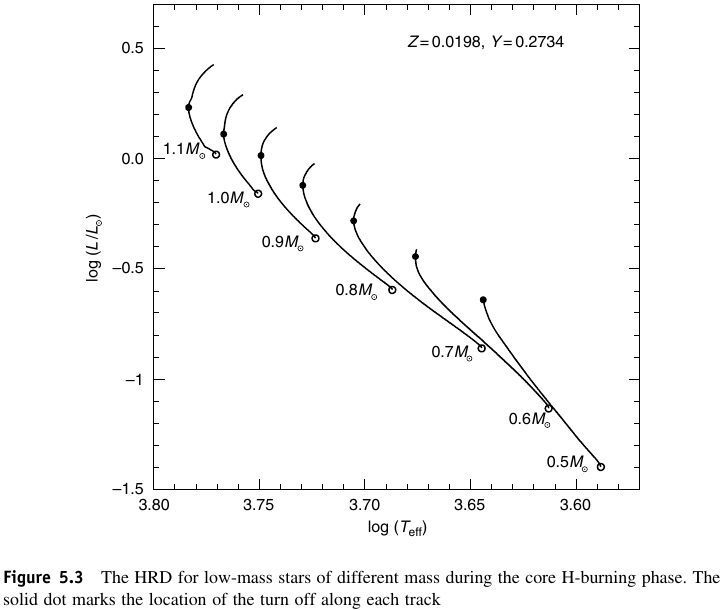
\includegraphics[trim={0cm 0cm 0 0},clip, keepaspectratio,width=0.99\textwidth]{HRD-LMS}\label{fig:HRD-LMS}
\end{figure}
\end{column}\begin{column}{0.6\textwidth}
La stella continua a contrarsi fino alla partenza della reazione $^3He(^3He,2^1H)^4He$ e il core convettivo svanisce con l'espandersi della regione in cui \'e prodotto $^3He$
Struttura: H-burn in central radiative core (Small T-dep of $\epsilon_{PP}$), convective core (large opacity associated to partial ionized H, He)
Evoluzione: $\#$ free particles $\downarrow$, \xaumenta{\mu} per HE \xaumenta{T}
, \xdiminuisce{R} quindi $L^*$ aumenta lentamente.
TO is hottest point in evolutionary track: H exhausted 
\end{column}\end{columns}
\end{frame}


\subsection{Upper main sequence ($M^*\geq1.2-1.3\msun{}$)}\linkdest{UMS}

\begin{frame}{Da ZAMS a Overall contraction}
\begin{columns}[T]\begin{column}{0.4\textwidth}
\begin{figure}[!ht]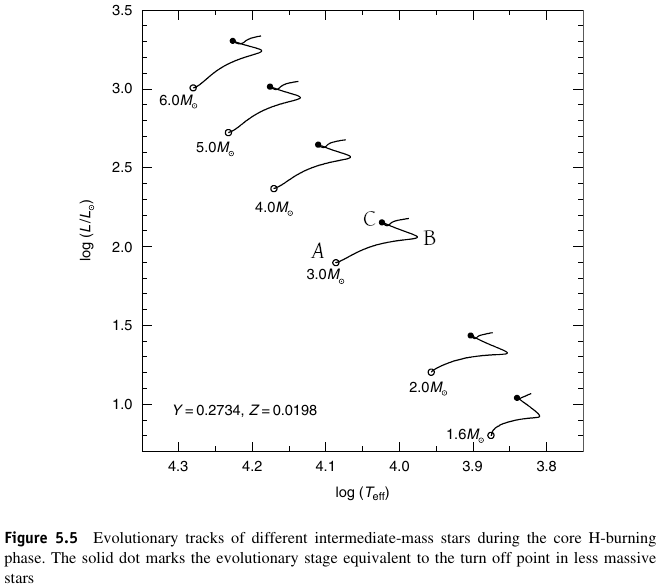
\includegraphics[trim={0cm 0cm 0 0},clip, keepaspectratio,width=0.99\textwidth]{HRD-UMS}\label{fig:HRD-UMS}
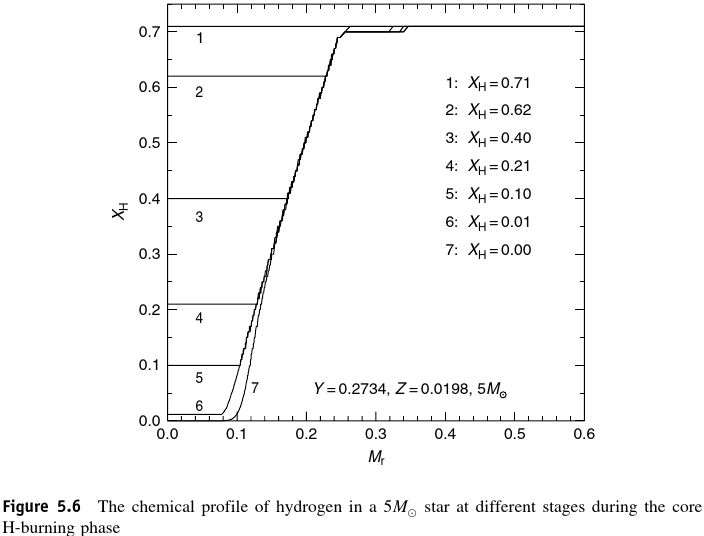
\includegraphics[trim={0cm 0cm 0 0},clip, keepaspectratio,height=0.42\textheight]{UMS-Hprofile}\label{fig:UMS-Hprofile}\end{figure}
\end{column}\begin{column}{0.6\textwidth}
\begin{block}{CNO H-Burning: convective core}
Higher T: CNO dominant: $\epsilon_{CNO}$ steeper:convective core: \xaumenta{M^*}, \xaumenta{M_{con}}, \xaumenta{P_{rad}}, \xdiminuisce{\nad{}}.
\end{block}
\begin{block}{As UMS burn H}
\begin{itemize}
    \item convective core shrink: ?\xaumenta{\mu}, \xaumenta{P_c}?
    \item radius expands: after H exhaustion
    \item core gravitationally contract
    \item $L$ increases such that $T_e$ has little drop
\end{itemize}
\end{block}
\begin{block}{Overall contraction}
When $X<0.05$ at B start gravitational contraction of core until C; after C inner regions contract outer expand
\end{block}
\end{column}\end{columns}
\end{frame}

\subsection{Deps of MS on Physical input}\linkdest{MSdeps}

\begin{frame}{Effects of changes in initial chemical composition}
\begin{block}{Different initial Y value: opacity and mean molecular weight}
\begin{columns}[T]
\begin{column}{0.5\textwidth}
\begin{figure}[!ht]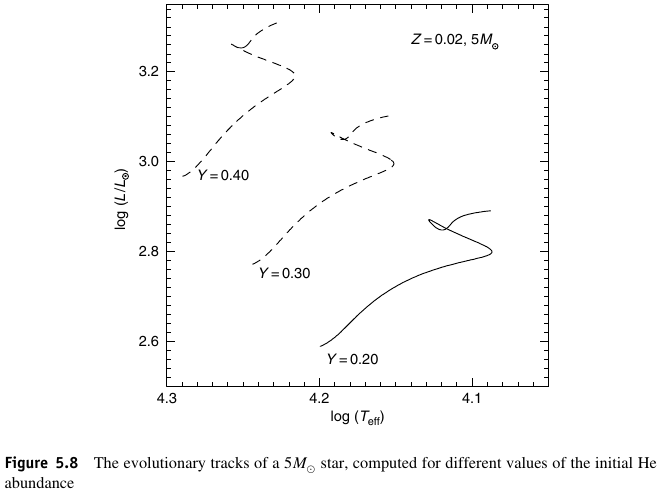
\includegraphics[trim={0cm 0cm 0 0},clip, keepaspectratio,width=0.99\textwidth]{HRD-changingHe}\label{fig:HRD-changingHe}
\end{figure}
\end{column}
\begin{column}{0.5\textwidth}
\begin{itemize}
    \item Increases of nuclear rates $L_H\propto\mu^7$
    \item Opacity decreases
\end{itemize}
Star is brighter and hotter
\end{column}
\end{columns}
\end{block}
\begin{block}{Changes in Z affect opacity}
\begin{itemize}
    \item \xaumenta{Z}, \xaumenta{\kappa}: fainter, cooler star.
    \item PP chain reaction not dependent on Z, CNO element are enough exept in pop III.
    \item $\alpha$-enhanced objects: CNO cycle efficiency increased, opacity increased with two bump at $\log{T}=6,5.5$ due to K shell O electrons and L-edges of Mg, Si, Ne. Stars are fainter and cooler
\end{itemize}
\end{block}
\end{frame}

\begin{frame}{Effects of changing convection efficiency: superadiabatic convection}
\begin{columns}[T]
\begin{column}{0.5\textwidth}
\begin{figure}[!ht]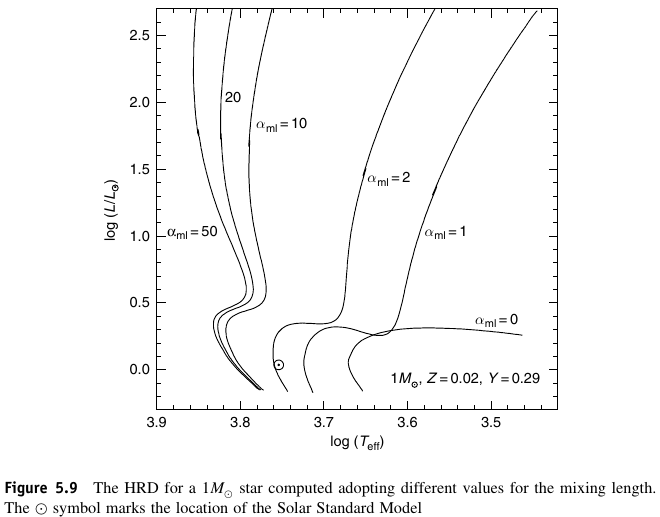
\includegraphics[trim={0cm 0cm 0 0},clip, keepaspectratio,width=0.99\textwidth]{HRD-1M-changingalpha}\label{fig:HRD-changingHe}
\end{figure}
\end{column}
\begin{column}{0.5\textwidth}
\begin{itemize}
    \item $\alpha_{ML}$ calibrated using Sun.
    \item $\alpha_{ML}$ does not affect L
    \item $\alpha_{ML}$ radius and $T_e$: \xaumenta{\alpha},\xdiminuisce{\nabla},\xaumenta{T_e},\xdiminuisce{R_s}
\end{itemize}
\end{column}
\end{columns}
\end{frame}

\begin{frame}{Convective core and Overshooting ($M>10\msun{}$)}
\begin{columns}[T]\begin{column}{0.5\textwidth}
\begin{figure}[!ht]
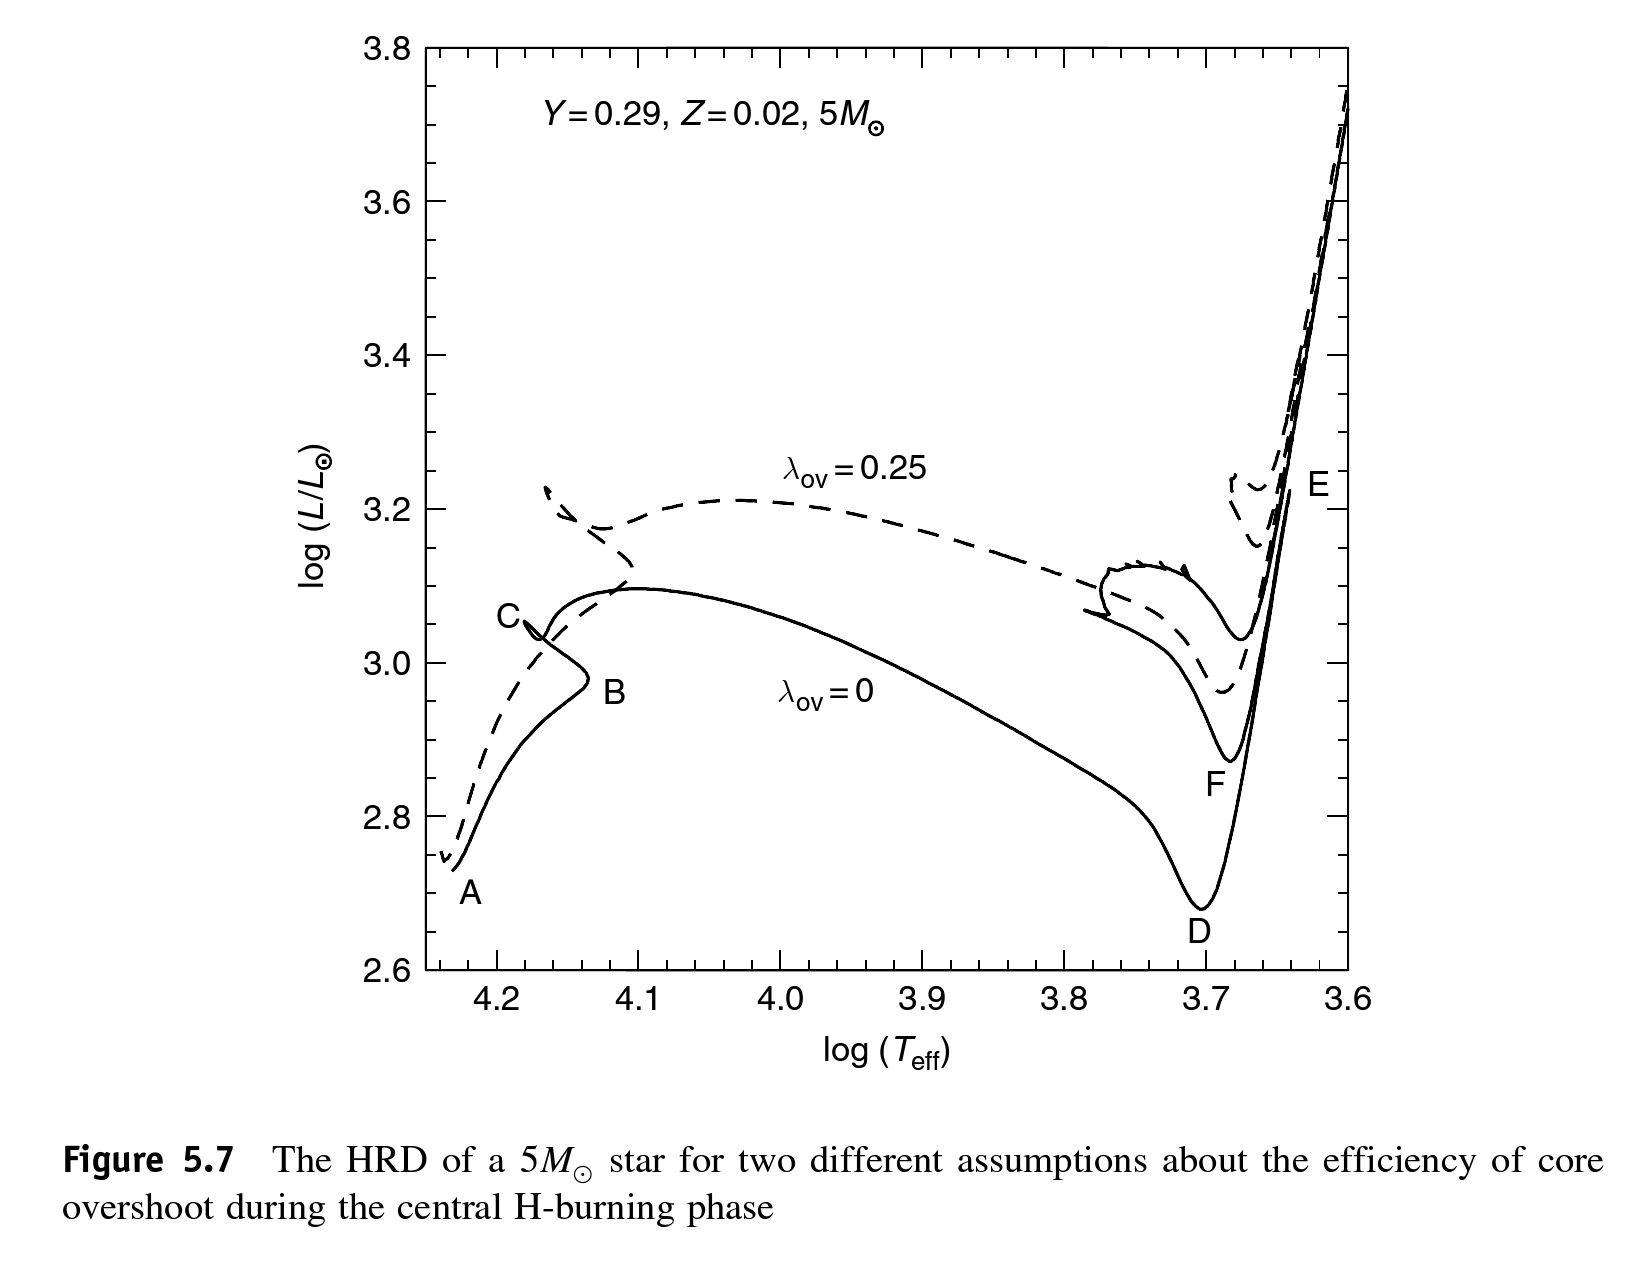
\includegraphics[trim={0cm 0cm 0 0},clip, keepaspectratio,height=0.42\textheight]{HRD-overshoot}\label{fig:HRD-overshoot}
\end{figure}
\end{column}
\begin{column}{0.5\textwidth}
\begin{block}{What increases convective core}
\begin{itemize}
\item Changes in physical input
\item Stellar rotation
\item Physical overshooting
\end{itemize}
\end{block}
\end{column}\end{columns}
\begin{columns}[T]\begin{column}{0.55\textwidth}
\begin{block}{Effects of increased convective core}
\begin{itemize}
\item \xaumenta{M_c}, \xaumenta{\mu} (involve more mass), \xaumenta{L}
\item Longer central H-burning
\item Larger He core at end of MS: brighter He-burning phase star, shorted lifetime
\end{itemize}
\end{block}
\end{column}
\begin{column}{0.45\textwidth}
\begin{block}{\sch vs Ledoux in-stability criterion}
In radiative region the retracting convective core leave chem composition gradient; but \xaumenta{He}, \xdiminuisce{\kappa}
\end{block}
\end{column}\end{columns}
\end{frame}

\begin{frame}{Low-mass star $M<0.4\msun{}$}
\begin{columns}[T]\begin{column}{0.4\textwidth}
\begin{figure}[!ht]
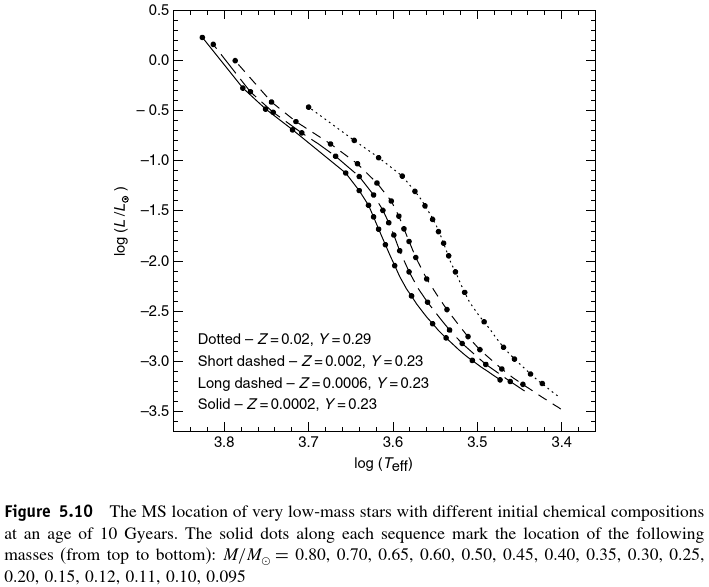
\includegraphics[trim={0cm 0cm 0 0},clip, keepaspectratio,width=0.99\textwidth]{VLM-HDR}\label{fig:VLM-HDR}
\end{figure}
\end{column}
\begin{column}{0.6\textwidth}
\begin{itemize}
    \item Fully convective through MS live
    \item PP1 H-burning with negligible $^3He$ destruction
    \item Transition between molecular H and atomic He to plasma at inner $90\%$ in mass: thermodynamical properties sensible to treatment of pressure ionizzation, dissociation, non-ideal Coulomb.
    \item Atmospheric features due to opacity sources: collisional induced dipole in $H_2$ molecules, CIA suppresses flux at \SI{2}{\micro\meter}; for $T_e<\SI{4000}{\kelvin}$ molecules of $TiO$ and $VO$ controll flux in optical, $H_2O$ and $CO$ the flux in infrared; for $T_e<\SI{2800}{\kelvin}$ also grains are important.
\end{itemize}
\end{column}\end{columns}
\end{frame}

\subsection{Mass-Luminosity relations}\linkdest{malure}

\begin{frame}{M-L relation}
Near ZAMS $L\propto M^3$. Assumption: radiative transport $L\propto\frac{R^4}{M}T^4$, HE $P\propto M^2/R^4$, perfect gas $P\propto\rho T$.
\begin{columns}[T]\begin{column}{0.5\textwidth}
\begin{figure}[!ht]
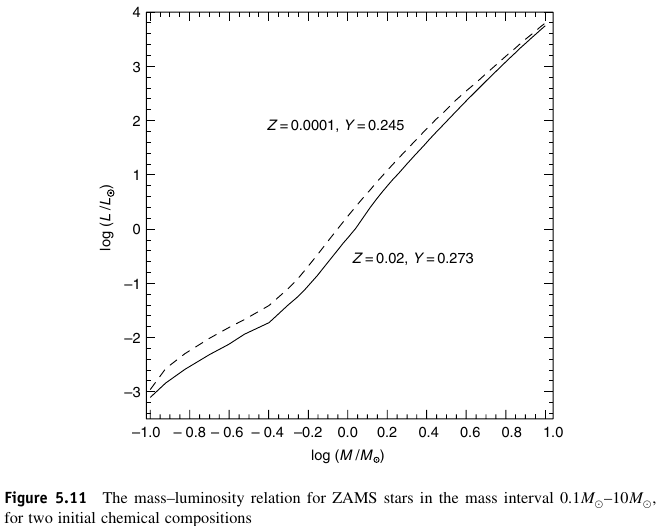
\includegraphics[trim={0cm 0cm 0 0},clip, keepaspectratio,width=0.99\textwidth]{ML-01-10}\label{fig:ML-01-10}
\end{figure}
\end{column}
\begin{column}{0.5\textwidth}
Relazione osservativa
\begin{equation*}
L\propto\begin{array}{l}
M,\ M>10\msun{}\\
M\expy{3.6},\ \numrange{2}{20}\msun{}\\
M\expy{4.5},\ \numrange{0.5}{2}\msun{}\\
M\expy{2.6},\ \numrange{0.2}{0.5}\msun{}\\
\end{array}
\end{equation*}
\end{column}\end{columns}
\end{frame}

\subsection{Post-MS: RGB??}\linkdest{postMS}
%SC [160]

\begin{frame}{Condizione Core per fusione}
\begin{figure}[!ht]
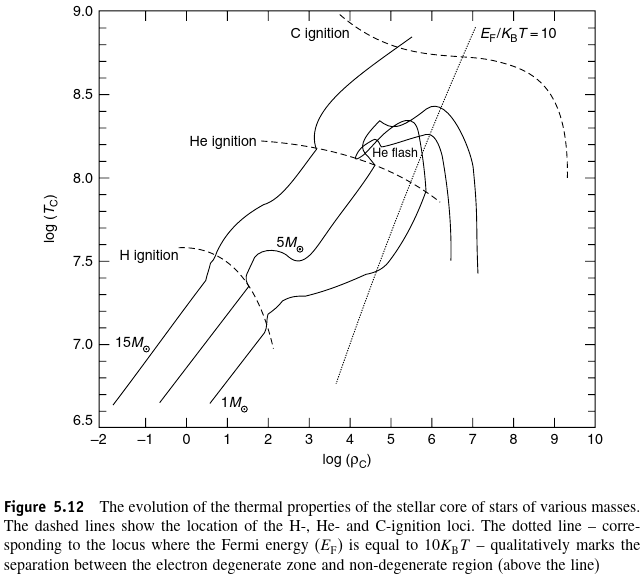
\includegraphics[trim={0cm 0cm 0 0},clip, keepaspectratio,height=0.4\textheight]{HHeCcore}\label{fig:HHeCcore}
\end{figure}
\begin{itemize}
    \item Electron degeneracy
    \item gravitational contraction: virial theorem
\end{itemize}
\end{frame}

\begin{frame}{SC-mass limit}
$L=0$ implica formazione core di He isotermo: se la massa del core di elio \'e maggiore del $10\%$ della massa totale della stella il core si contrae - le stelle della LMS hanno core pi\'u piccolo, stelle di massa $M\geq2.5-3\msun{}$  hanno core pi\'u grande.
\begin{equation*}
\frac{M_c}{M}>(\frac{M_c}{M})_{SC}=0.37(\frac{\mu_{env}}{\mu_c})^2\xrightarrow{\parbox{2.5cm}{$\mu_e=\mu_{\odot}=0.6$\\$\mu_c=\mu(He)=1.3$}}0.08
\end{equation*}
il core si contrae su $\tkh{}$.
Virial theorem for non-vanishing pressure surface pressure $P_0$ and $M_c$, $R_c$ and $T_c$:
\begin{align*}
&(2U_i+\Omega+S_p=0,\ S_p=-\int\exv{v^2}\Vec{r}\cdot\hat{n}\,dS=P_0V)\\
&P_0=K_1\frac{M_cT_c}{R_c^3}-K_2\frac{M_c^2}{R_c^4}\\
&P_{0,m}=K_3T_c^4/M_c^2
\end{align*}
For equilibrium $P_{0,m}\geq P_e\propto M_t^2/R^4=T_c^4/M_t^2$ ($T_c\propto M_t/R$)
\end{frame}

\begin{frame}{Int-massive stars: from SG to RG}
\begin{columns}[T]\begin{column}{0.44\textwidth}
\begin{figure}[!ht]
%trim: LBRT
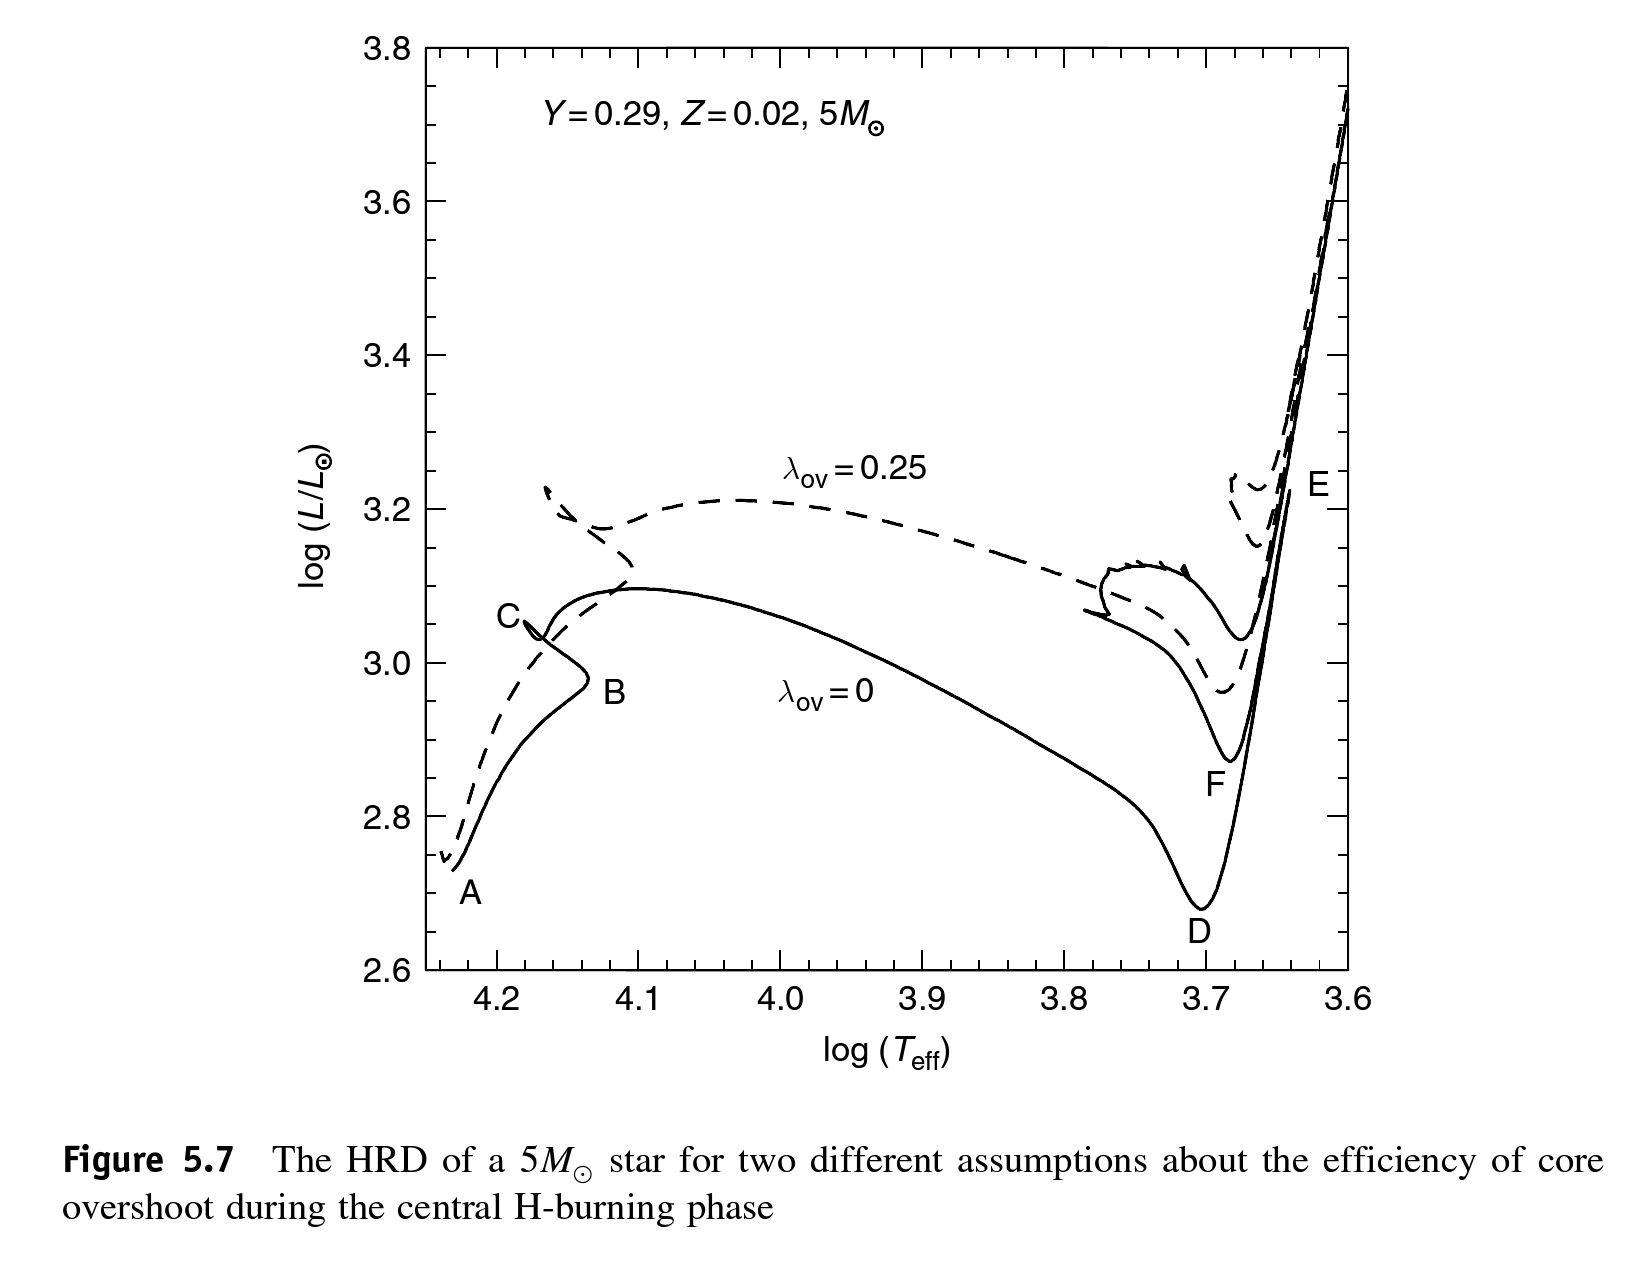
\includegraphics[trim={2cm 2cm 3cm 1cm},clip, keepaspectratio,width=0.99\textwidth]{HRD-overshoot}\label{fig:HRD-overshoot}
\end{figure}
\end{column}
\begin{column}{0.55\textwidth}
\begin{itemize}
    \item $M_c>M_{SC}$ ($M\approx2.3-3$ dopo H-burning in shell): He core contract
    \item broad shell of CNO H-burning: $\epsilon_g$ changes sign at max $\epsilon_{CNO}$ - envelope expand: \xdiminuisce{T_e}, \xaumenta{\kappa_e} quindi inviluppo diventa convettivo.
    \item Star move from B to R at constant L - Hertzsprung gap: $\begin{array}{c}\tkh{}(3\msun{})\approx\SI{12}{\mega\year}\\\tkh{}(6\msun{})\approx\SI{1}{\mega\year}\end{array}$
\end{itemize}
\end{column}\end{columns}
\begin{itemize}
    \item In (D) star reaches Hayashi track where begins RG phase: $T_e$ costante, \xaumenta{L}
    \item $\rho_c$ suff. low such onset of \Pelectron degeneracy is avoided: in (E) contracting core reaches $T\approx\SI{e8}{\kelvin}$ for efficient He-burning. \xaumenta{M_c} (VT: \xaumenta{T_c}) \xdiminuisce{\tau_{RG}}
\end{itemize}
\end{frame}

%trim: LBRT
\begin{frame}{Low-mass stars}
\begin{columns}[T]\begin{column}{0.44\textwidth}
\begin{figure}[!ht]
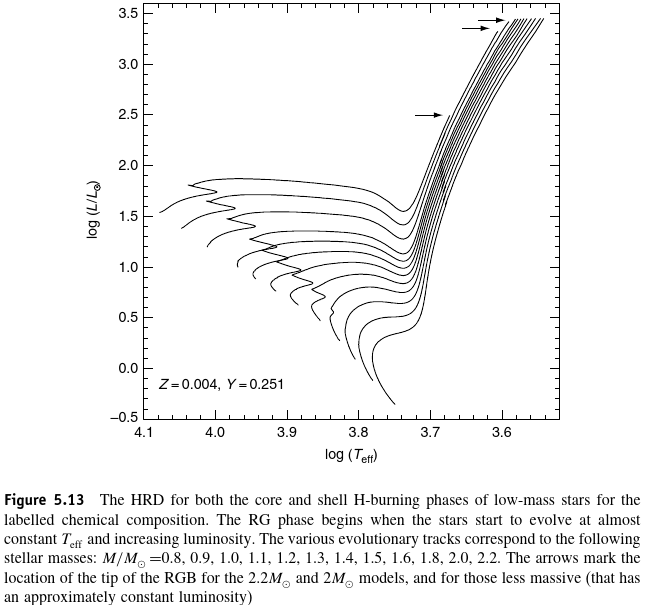
\includegraphics[trim={0cm 0cm 0cm 0cm},clip, keepaspectratio,width=0.99\textwidth]{HDRtipRGB}\label{fig:HDRtipRGB}
\end{figure}
\end{column}
\begin{column}{0.55\textwidth}
\begin{itemize}
\item As X exhausts max $\epsilon_H$ is no more in central region (at TO at $M_r=0.1\msun{}$). He Core (radiative/small convective??): $M<M_{SC}$, high electron degeneracy.
\item From TO to RG H-burning shell becomes thinner due to CNO deps on T that decreses in envelop and to X exhaustion.
\end{itemize}
\end{column}\end{columns}
\begin{itemize}
\item $M_{cHe}-L$ relation: \xaumenta{M_{cHe}}, \xaumenta{L}. L is almost fully provided by H-burning shell whose thermal properties are determined $R_c$, $M_c$ ($P_e$ is OM lower)
\item RGB stars evolve at constant L and radius re-adjust to stellar mass: mass loss shift $T_e$ toward lower values.
\end{itemize}
\end{frame}

\begin{frame}{Envelop structure: depth of convection and first dredge-up}
\begin{columns}[T]\begin{column}{0.44\textwidth}
%trim: LBRT
\begin{figure}[!ht]
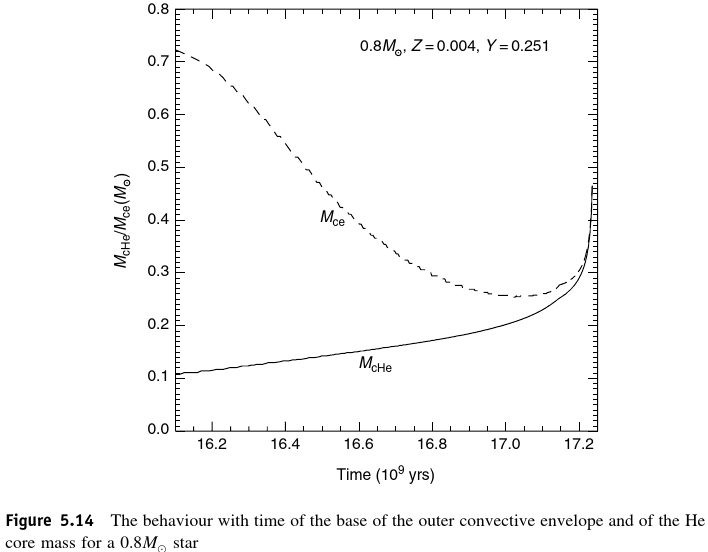
\includegraphics[trim={0cm 0cm 1cm 0cm},clip, keepaspectratio,height=0.35\textheight]{postMS-depthC}\label{fig:postMS-depthC}
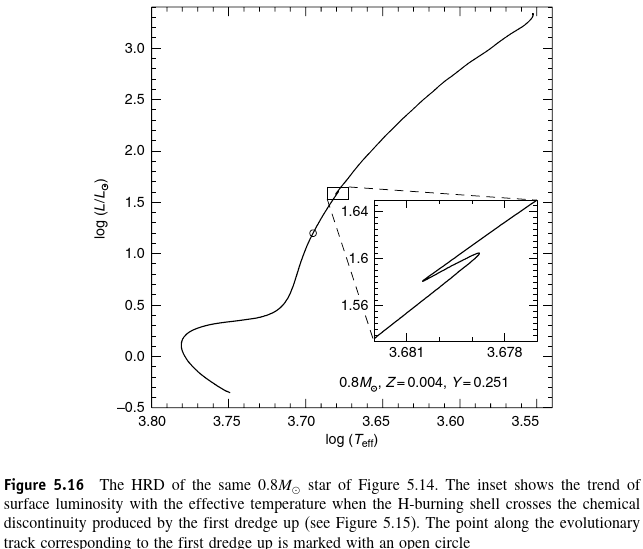
\includegraphics[trim={0cm 0cm 1cm 0cm},clip, keepaspectratio,height=0.35\textheight]{HburnxIdu}\label{fig:HburnxIdu}
\end{figure}
\end{column}
\begin{column}{0.55\textwidth}
\begin{itemize}
\item Cooling of envelop causes deeper convection that reaches a maximum before RG (\xdiminuisce{T}, \xaumenta{\kappa}). Primo dredge-up: \xaumenta{He_s}, \xaumenta{^{14}N_s}, \xdiminuisce{^{12}C} ($\frac{^{12}C}{^{13}C}$), $Li$, $Be$ reduces several OM.
\item In RGB phase H-burning shell move outward and convective zone move toward surface: chemical discontinuity at max convective depth. \keyword{Bump of RGB}: as H-burning shell meet discontinuity $L_H\propto\mu^7$ diminish the in fully mixed envelop \xaumenta{L} as \xaumenta{M_{cHe}} - bump in RGB luminosity function ($20\%$ rgb-time in this luminosity range)
\end{itemize}
\end{column}\end{columns}
\end{frame}

\begin{frame}{\keyword{Thermal runaway at tip of RGB}: He-flashes}
\begin{columns}[T]\begin{column}{0.44\textwidth}
%trim: LBRT
\begin{figure}[!ht]
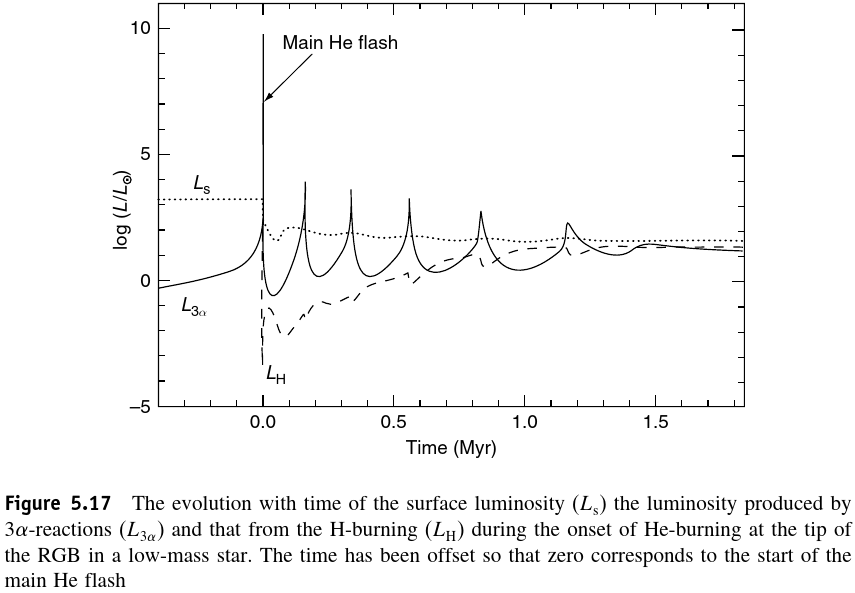
\includegraphics[trim={0cm 0cm 1cm 0cm},clip, keepaspectratio,width=0.99\textwidth]{He-flash}\label{fig:He-flash}
\end{figure}
\end{column}
\begin{column}{0.55\textwidth}
In RG phase: H-burning increases $M_{cHe}$ and \xaumenta{\rho_c}. In inner part $M_r<0.3M_t$ when $\epsilon_g+\epsilon_{\nu}<0$: $\TDy{r}{L}<0$ resulting in T-inversion. \xaumenta{\rho_c}, grado di degenerazione aumenta, \xdiminuisce{\kappa_{cond}}, \xdiminuisce{T_c}; while \xaumenta{T_c^M} due to $\epsilon_g>0$ at boundary between D/ND matter. At $T_c^M\approx\SI{e8}{\kelvin}$ we have He ignition ($M_{cHe}\approx0.48-0.5\msun{}$): end of RGB phase.
\end{column}\end{columns}
He ignition at strong partial-relativistic-D ($\rho_x\approx\SI{e6}{\gram\per\cubic\cm}$, $T\approx\SI{8e7}{\kelvin}$), $P$ is insensitive to $T$ changes, rate of $3\alpha$-burning increases much: thermal runaway $\num{e10}\lsun{}$ in few seconds are absorbed by above ND layers: expansion and convection (large jump in P/S prevent mixing with above H-burning). So \xaumenta{T} at constant $\rho$ but no time for heat diffuse the whole core: this need many successive He-flashes, $\tau_{flash}\approx\SI{e6}{\year}$ and $5\%$ He converted to C
\end{frame}

\begin{wordonframe}{SC: WD cooling $[22], [45]$, Z poor $[196]$}

\end{wordonframe}

\subsection{Deps of RGB on params}\linkdest{depsRGB}

\begin{frame}{Location of RGB on HRD}
\begin{itemize}
\item Highly Z-dependent: size of convective envelop (Hayashy track) \xaumenta{Z}, \xaumenta{\kappa}, inviluppo convettivo pi\'u grande:  $\alpha$-enhanced stars (more low ionization potential: Mg, Si, ...) form molecule $TiO$ and $H^-$: RGB cooler and less steeper.
\item \xaumenta{Y}, \xdiminuisce{\kappa}, \xdiminuisce{CE}, \xaumenta{T_e}
\item RGB is important Z indicator of galaxies/star clusters
\item $\rho_e$ low: $\nabla_e$ \'e super-adiabatico (\xaumenta{
\alpha_{ML}},\xaumenta{T_e})
\item \keyword{RGB phase transition}. \xdiminuisce{M_*}, \xdiminuisce{T_e}: $M_{cHe}$ constant for $M\leq1.8\msun{}$ then decreases with $M$ as degeneracy is completely removed 
\end{itemize}
\end{frame}

\begin{frame}{Deps RGB's L-bump on params}
\begin{columns}[T]\begin{column}{0.55\textwidth}
%trim: LBRT
\begin{figure}[!ht]
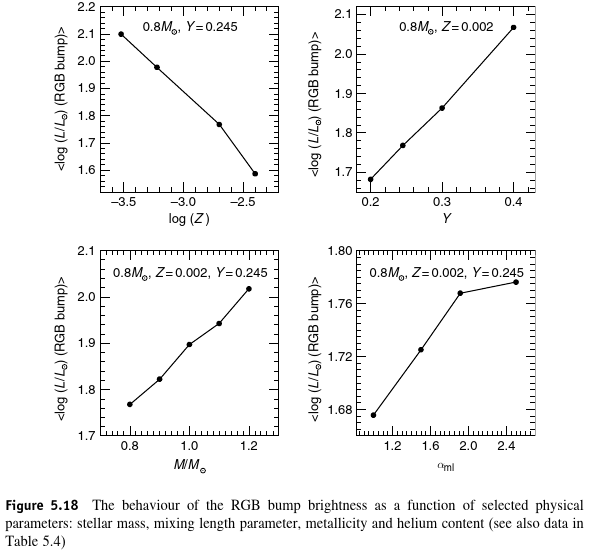
\includegraphics[trim={0cm 0cm 1cm 0cm},clip, keepaspectratio,width=0.99\textwidth]{RGB-bumpparams}\label{fig:RGB-bumpparams}
\end{figure}
\end{column}
\begin{column}{0.45\textwidth}
As convection zone goes deeper the H-burning shell takes less time to cross chemical discontinuity: (\xdiminuisce{M_*}/\xaumenta{Z}/\xdiminuisce{Y},\xdiminuisce{\alpha_{ML}}), \xdiminuisce{L_{bump}}
\end{column}\end{columns}
\end{frame}

\begin{frame}{Deps RGB tip's (He-ignition) luminosity on params}
\begin{columns}[T]\begin{column}{0.44\textwidth}
%trim: LBRT
\begin{figure}[!ht]
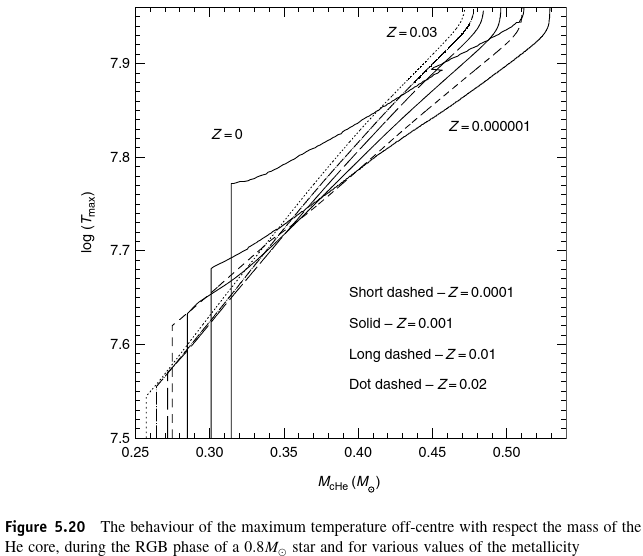
\includegraphics[trim={0cm 0cm 1cm 0cm},clip, keepaspectratio,height=0.36\textheight]{RGBTmax}\label{fig:RGBTmax}
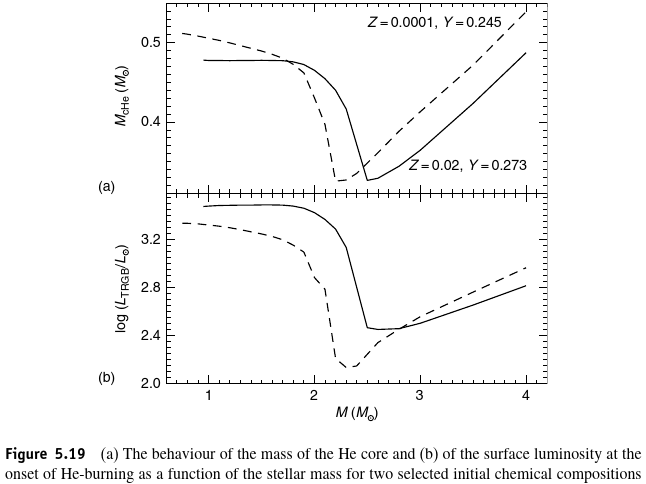
\includegraphics[trim={0cm 0cm 1cm 0cm},clip, keepaspectratio,height=0.36\textheight]{HecLsatHeburning}\label{fig:HecLsatHeburning}
\end{figure}
\end{column}
\begin{column}{0.55\textwidth}
\begin{itemize}
    \item \keyword{RGB phase transition}. \xdiminuisce{M_*}, \xdiminuisce{T_e}: $M_{cHe}$ constant for $M\leq1.8\msun{}$ then decreases with $M$ as degeneracy is completely removed then increases as consequences of larger convective H-burning core.
    \item \xaumenta{He}, \xaumenta{T_c}, deg \Pelectron diminuisce, $M_{cHe}$ He-ignition diminuisce, \xdiminuisce{L_{TIP}}
    \item \xaumenta{Z}, \xaumenta{\epsilon_{CNO}}, $M_{cHe}$-ignition is builded faster since He production is faster and He-core heating is faster, \xaumenta{L_{TIP}}
\end{itemize}
\end{column}\end{columns}
\end{frame}

\subsection{Very low Z stars}\linkdest{lowz}

\begin{frame}{Very low Z (pop III)}
\begin{itemize}
    \item Primordial star (Pop III) responsable for Z-enrichment: from $Z\approx\numrange{e-10}{e-12}$ to $Z\approx\numrange{e-2}{e-3}$ (Pop II)
    \item High mass star burn H through PP chain so need much higher T; as $T\approx\SI{e8}{\kelvin}$ He-burning produce $^{12}C$: threshold for CNO H-burning to begins $X_C\approx\numrange{e-9}{e-10}$
    \item \xaumenta{M_*}, \xdiminuisce{\tau_{PP\to CNO}}: transition to convective core for $M>2\msun{}$ (for $M=2-5\msun{}$ convective core after $^3He$ production phase).
    \item RGB phase transition at lower mass/higher age: for low mass star \xaumenta{T_c}, degenerazione elettronica del core di He diminuisce, faster He ignition, \xdiminuisce{M_{cHe}}, \xdiminuisce{L_{TIP}}
    \item Intermediate mass star have no RGB
\end{itemize}
\end{frame}

\subsection{Combustione He in nucleo di He non degenere}\linkdest{ZAHB}

\begin{frame}{Memo per HB}
combustion di He per stelle medio-grandi; clump He; loop He; Esaurimento He centrale: , semiconvezione e pulsi convettivi
\end{frame}

\begin{frame}{He-burning reactions}
	\begin{align*}
	&3\alpha (T\gtrsim\SI{1.2e8}{\kelvin}):\\ &^4He+^4He\to^8Be\tag*{$\tau_{1/2}\approx\SI{e-16}{\second}$}\\
	&^8Be+^4He\to^{12}C+\gamma\tag*{$\SI{7.27}{\mega\ev}$, $\tau_H\approx100\tau_{He}$}\\
	&\epsilon_{3\alpha}\approx\begin{array}{c}T^{40}: T\approx\SI{e8}{\kelvin}\\T^{20}: T\approx\SI{2e8}{\kelvin}\end{array}\\
	&^{12}C+\alpha\to^{16}O+\gamma\\
	&^{16}O+\alpha\to^{20}Ne+\gamma\\
	&^{20}Ne+\alpha\to^{24}Mg+\gamma\\
	&^{24}Mg+\alpha\to^{28}Si+\gamma
	\end{align*}

\end{frame}

\begin{frame}{ZAHB: equilibrium model}
\begin{itemize}
\item $\tau_{He-Flash}\approx\SI{e6}{\year}$: after that time of He-burning the \Pelectron degeneracy is removed (small obser. prob). Some authors start He-core evolution sequence from C enriched equilibrium model
\item \keyword{ZAHB}: model where He is burnt into chem homo-core and H in shell with chem stratification He-flash like
\item He-enriched by I dredge-up
\item Rotation (dalayed He-flash): \xaumenta{M_{cHe}}, \xdiminuisce{M_*} (mass loss), \xaumenta{T^{ZAHB}}/\xaumenta{L^{ZAHB}}
%\xaumenta{\epsilon_{He}}/\xdiminuisce{\epsilon_H}
\end{itemize}
\end{frame}

\begin{frame}{ZAHB in HDR}
\begin{columns}[T]
	\begin{column}{0.55\textwidth}
		\begin{itemize}
			\item 
		\end{itemize}
	\end{column}
	\begin{column}{0.45\textwidth}
		\begin{figure}[!ht]
			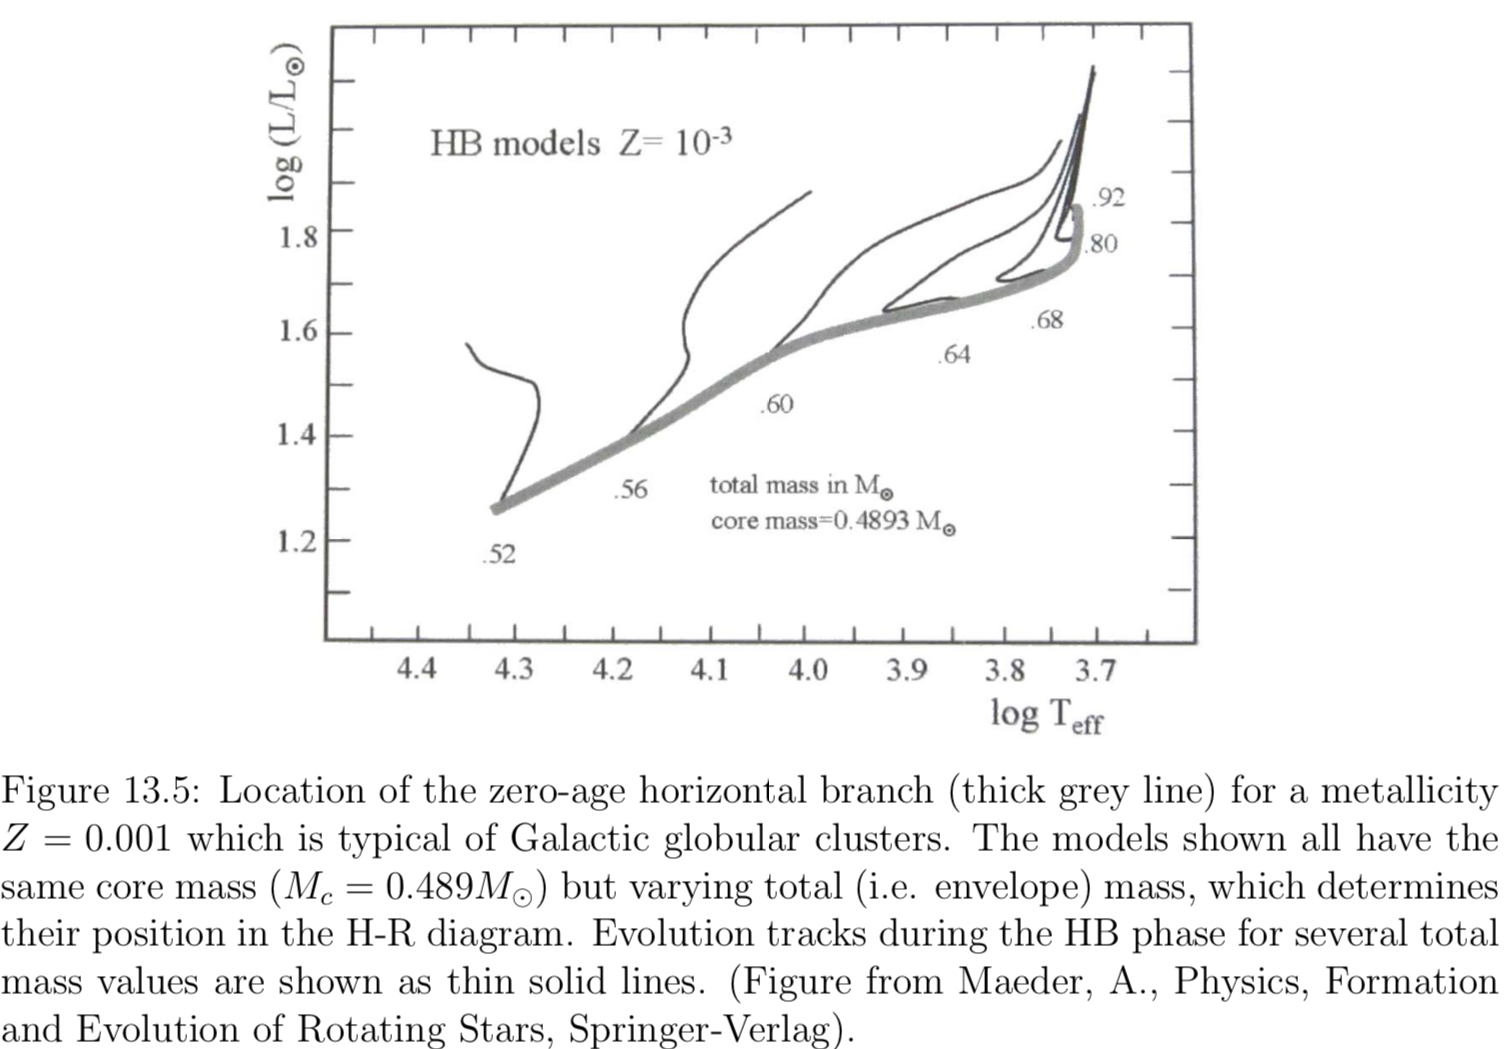
\includegraphics[trim={0cm 0cm 1cm 0cm},clip, keepaspectratio,height=0.37\textheight]{HB-ZA-evol}\label{fig:HB-ZA-evol}
		\end{figure}
	\end{column}
\end{columns}
\end{frame}

\begin{frame}{ZAHB dep on core (and envelope) mass}
\begin{itemize}
\item Structure and evolution of ZAHB fixed by: $M_*$, $M_{cHe}$ (for $M<1.8\msun{}$ $t_{TIP}>4-5\si{\giga\year}$: $M_c$ weakly dependent on M), $Y$, $Z_e$ - For fixed composition, $L_s$ is fixed by $M_{cHe}$ (then by $M_e$): important standard candles for Pop II stars (\keyword{Standard candles: HB brightness}). $(\TDy{M_{cHe}}{\log{L_{ZAHB}^{\log{T_e}=3.85}}})_{Y,Z}\approx3.04$
\item Location in HDR: \xdiminuisce{M_e}, \xaumenta{T_e} - HB (slightly oblique due to \xaumenta{\epsilon_H},\xaumenta{M_e}). $T_e\approx\SIrange{3500}{4000}{\kelvin}$ for $M_e\approx\numrange{e-4}{0.4}\msun{}$ (RGB mass loss)
\item \xaumenta{R_{cHe}}, \xdiminuisce{L_s} from RGB-tip as H-burning shell cool down
\item He-burning in convective core (steep T deps)
\item H-burning in shell: for fixed $M_{cHe}$ efficiency determined by \xaumenta{M_e}, \xaumenta{\epsilon_H}
\end{itemize}
\end{frame}

\begin{frame}{ZAHB dep on composition}
\begin{columns}[T]
\begin{column}{0.55\textwidth}
\begin{itemize}
\item \xaumenta{Y_{in}}, \xdiminuisce{M_{cHe}}, \xaumenta{L_H}/\xdiminuisce{L_{cHe}}, $L^{ZAHB}$ approx const: B part of ZAHB becomes fainter/ R part brighter. $(\TDy{Y}{L_{ZAHB}^{3.85}})_{M_{cHe},Z}\approx2.07$
\item \xaumenta{Z_{in}}, \xdiminuisce{M_{cHe}^{Flash}}/\xaumenta{\kappa_e}, \xdiminuisce{L^{ZAHB}}/\xdiminuisce{T_e^{ZAHB}}. $(\TDy{Z}{L_{ZAHB}^{3.85}})_{M_{cHe},Y}\approx-0.04$
\end{itemize}
\end{column}
\begin{column}{0.45\textwidth}
\begin{figure}[!ht]
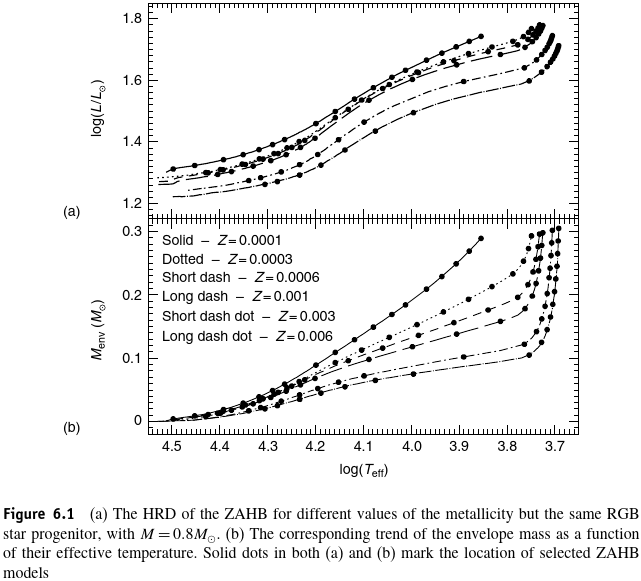
\includegraphics[trim={0cm 0cm 1cm 0cm},clip, keepaspectratio,height=0.37\textheight]{HDR-ZAHB-M08}\label{fig:HDR-ZAHB-M08}
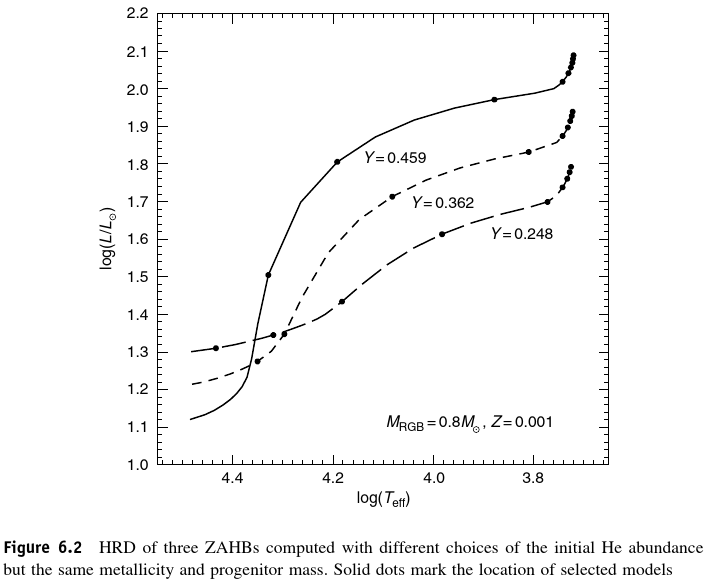
\includegraphics[trim={0cm 0cm 1cm 0cm},clip, keepaspectratio,height=0.37\textheight]{HDRZAHBdiffY}\label{fig:HDRZAHBdiffY}
\end{figure}
\end{column}
\end{columns}
\end{frame}

\subsection{Core He-burning in low-mass stars}\linkdest{HBlowM}

%\TDy{}{}=\alpha\frac{dP}{P}-\delta\frac{dT}{T}+\phi\frac{d\mu}{\mu}
%dq=c_PdT-\frac{\delta}{\rho}\,dP
\begin{frame}{HB evolution in HDR}
\begin{columns}[T]
\begin{column}{0.5\textwidth}
\begin{itemize}
\item \xaumenta{\epsilon_{He}}, \xdiminuisce{\epsilon_H}: as $L_{He}<L_H$ star evolves at \xaumenta{T_e}, $L_{He}>L_H$ star moves toward R. (Loop)
\end{itemize}
\end{column}
\begin{column}{0.5\textwidth}
\begin{figure}[!ht]
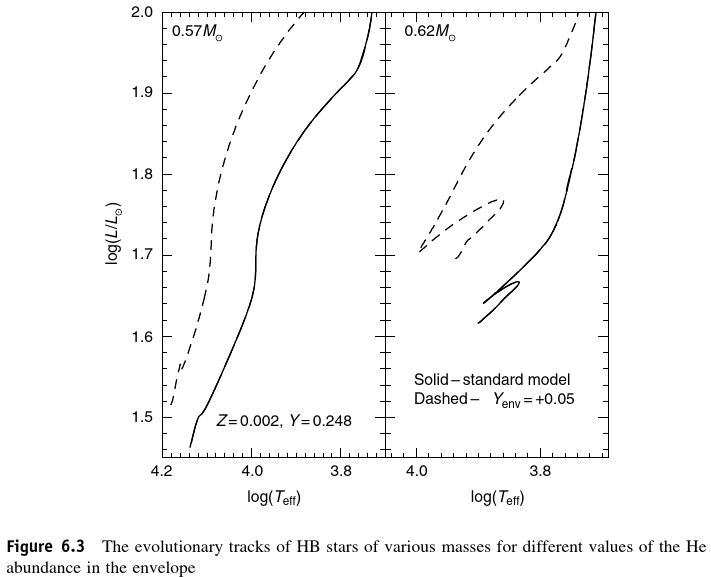
\includegraphics[trim={0cm 0cm 1cm 0cm},clip, keepaspectratio,height=0.37\textheight]{HB-lowM-evol}\label{fig:HB-lowM-evol}
\end{figure}
\end{column}
\end{columns}
\end{frame}

\begin{frame}{Mixing processes and physical properties evolution}
\begin{block}{Convective instability}
Mixing processes in convective He-burning core: $\tau_{con}\ll\tau_{nuc}$, as $^4He\to^{12}C$, \xaumenta{\kappa_{ff}} ($\propto X_iZ_i^2$), \xaumenta{\nrad{}} - growing discontinuity in T gradient at convective core boundary - overshoot cause mixing with radiative shell: \xaumenta{\kappa} - convective instability of boundary - selfdriving mechanism for extension of convective core - Convective boundary is established where $\nabla_{ad}=\nabla_{rad}$
\end{block}
\begin{block}{semi-convection}
$\nrad{}$ show a minimum due to outward shift in He-rich environment (complex behaviour of $\nrad$ due to local L, T, $\kappa$, P) - physical/chemical coupling convective zone outside minimum and mass of surrounding radiative layers - mixing of radiative shell: \xdiminuisce{\nad{}} in convective envelope (He-rich matter/properties of mixed shell) - convective core/convective shell not fully mixed: extended partially mixed semi-convection zone outside convective core between $\nrad$ minimum and radiative region
\end{block}
\end{frame}

\begin{frame}{Evolution of radiative gradient and convective zones boundaries in HB}
\begin{columns}[T]
\begin{column}{0.5\textwidth}
\begin{itemize}
\item Growing discontinuity of $\nrad$ at boundary of convective core for He-burning star low mass star as stellar model evolve from 1 to 5
\item (a) with increasing chem discontinuity; (b) convective overshoot
\end{itemize}
\end{column}
\begin{column}{0.5\textwidth}
\begin{figure}[!ht]
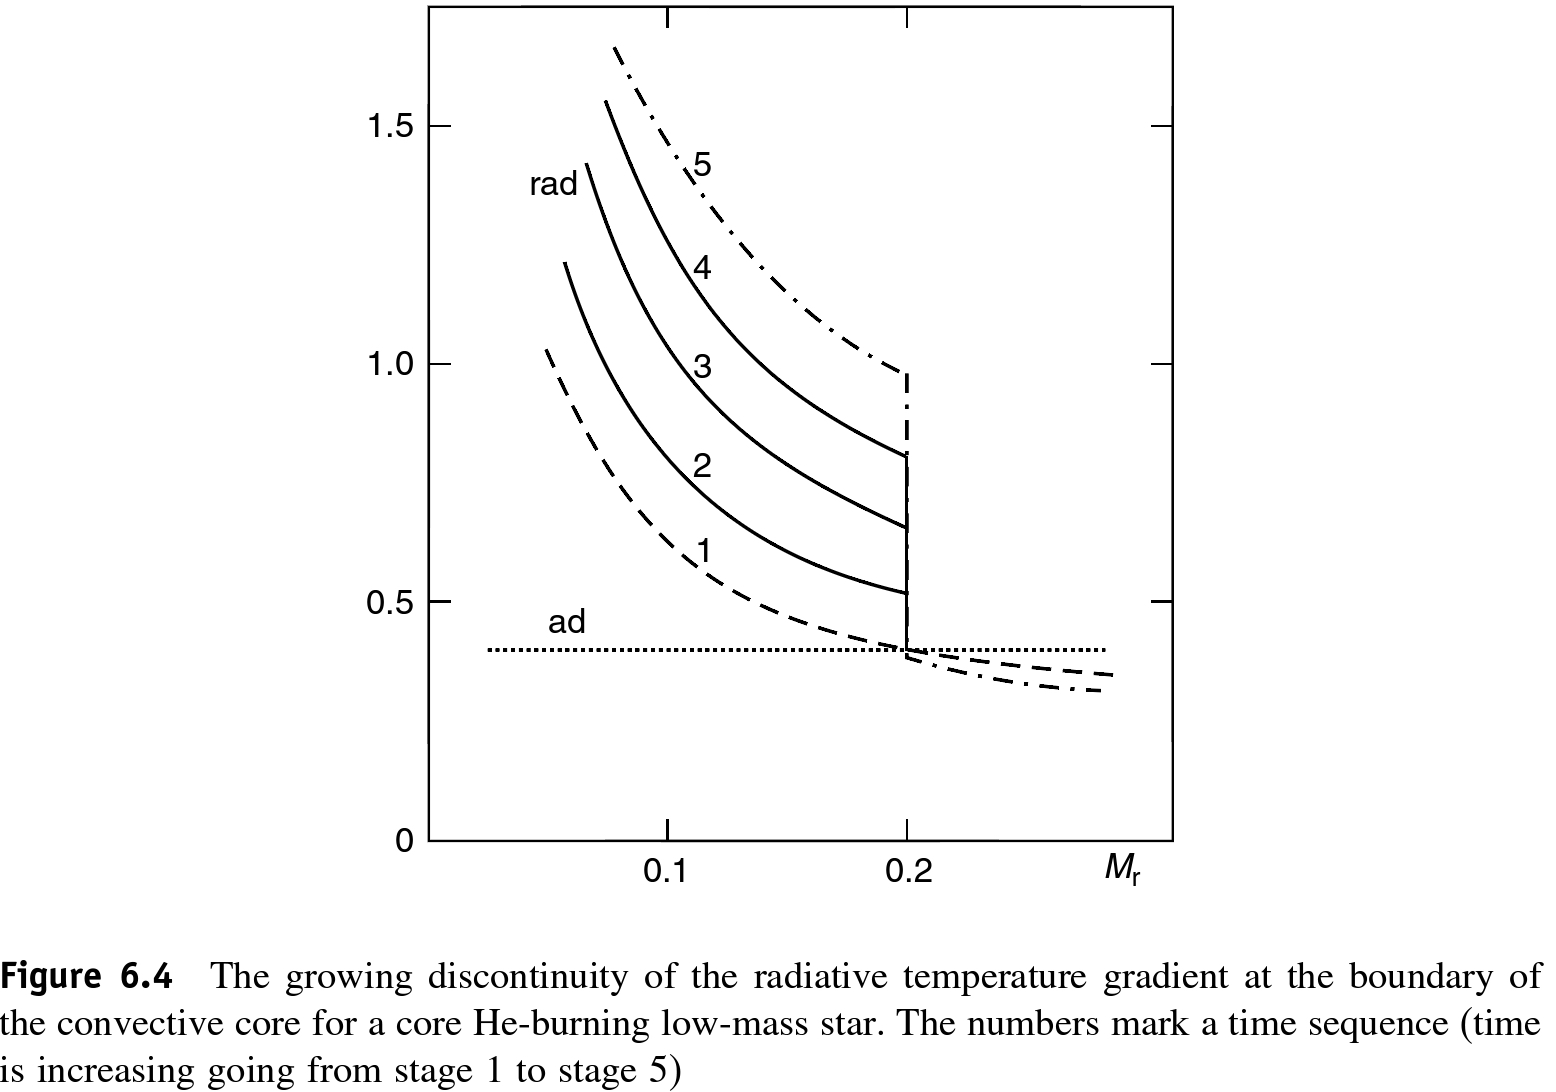
\includegraphics[trim={0cm 0cm 1cm 0cm},clip, keepaspectratio,height=0.4\textheight]{HBnrad-seq}\label{fig:HBnrad-seq}	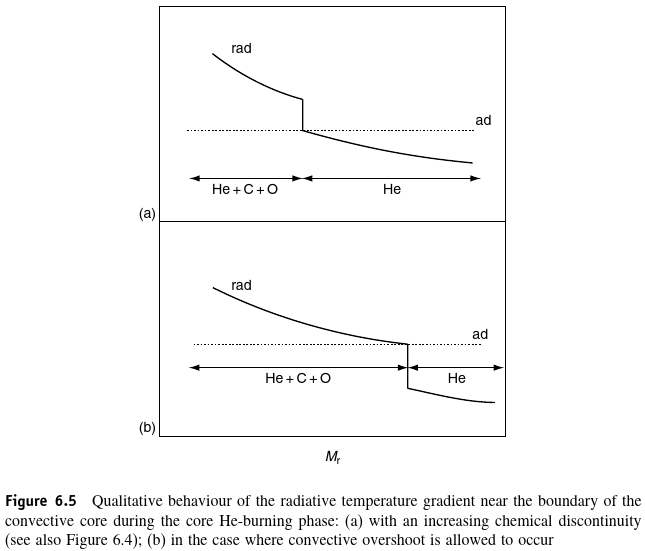
\includegraphics[trim={0cm 0cm 1cm 0cm},clip, keepaspectratio,height=0.4\textheight]{HBnablaraddisos}\label{fig:HBnablaraddisos}
\end{figure}
\end{column}
\end{columns}
\end{frame}

\begin{frame}{Semi-convective region}
\begin{columns}[T]
\begin{column}{0.5\textwidth}
\begin{itemize}
\item Time sequence which result in appearance of semi-convection region
\end{itemize}
\end{column}
\begin{column}{0.5\textwidth}
\begin{figure}[!ht]
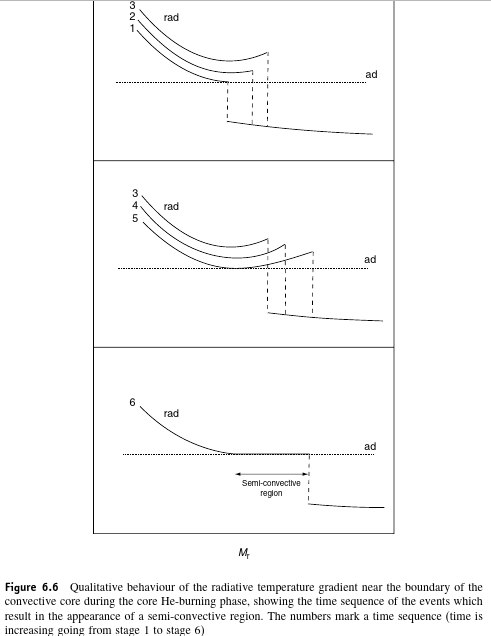
\includegraphics[trim={0cm 0cm 1cm 0cm},clip, keepaspectratio,width=0.99\textwidth]{HBnablaraddiscsc.png}\label{fig:HBnablaraddiscsc.png}
\end{figure}
\end{column}\end{columns}
\end{frame}

\begin{frame}{Breathing pulse and observative consequences}
\begin{columns}[T]
	\begin{column}{0.55\textwidth}
	\begin{itemize}
		\item Core convective instability - 3 breathing pulses are needed to completely exhaust He in core: when $Y_c\approx0.1$ occurs core convective instability - when $^{12}C+\alpha\to^{16}O$ overcome $^{12}C$ production by $3\alpha$ \xaumenta{\kappa} quindi aumenta la dimensione della zona convettiva quindi \xaumenta{Y_c}, \xaumenta{L}(\xaumenta{\epsilon_{He}}), \xaumenta{\nrad}, aumenta zona convettiva (\keyword{breathing pulses}: after each pulse star readjust to burn He steadly)
		\item Effects of BP - i) Loop in HDR at each pulse ii) He burning time increased iii) $M_{cc}$ increased
	\end{itemize}
	\end{column}
	\begin{column}{0.45\textwidth}
	\begin{figure}[!ht]
	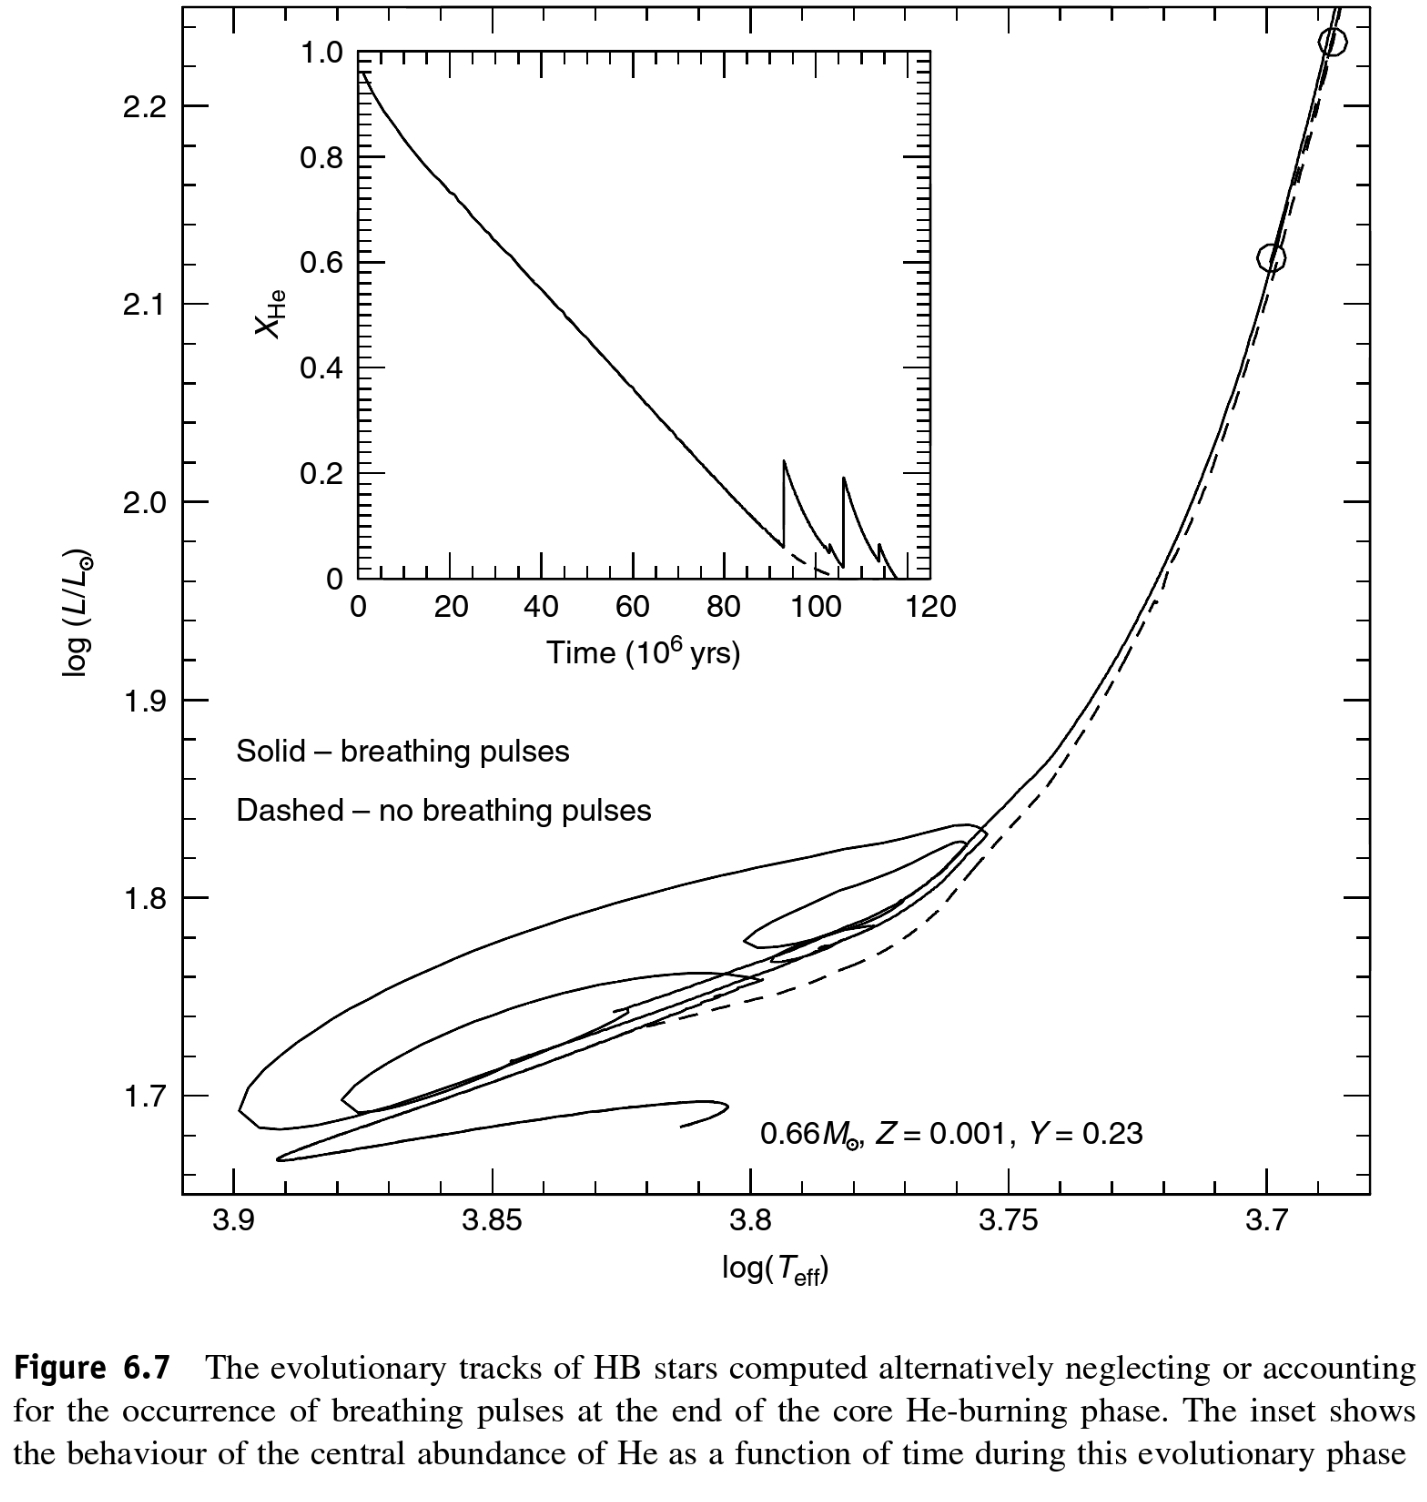
\includegraphics[trim={0cm 0cm 1cm 0cm},clip, keepaspectratio,width=0.99\textwidth]{HBbreathing}\label{fig:HBbreathing}
	\end{figure}
\end{column}\end{columns}
	\begin{itemize}
	\item R2 parameter - ratio of number of star in AGB to stars in HB (lifetime ratio)  $=0.12-0.15$ without BP, $0.8-0.14$ with BP - observed R2 in globular cluster ([36], [44]): BP efficiency very low, BP could be due to breakdown in instantaneous mixing approx in stellar models when convection setin in late HB stages
\end{itemize}
\end{frame}

\begin{frame}{Discussioni parametri che influenzano HB}
Parametro R per determinazione He
\end{frame}

\subsection{Core He-burning in Int/Mas stars}\linkdest{HBIM}

\begin{frame}{Evolution in HDR during HB for Int./massive star}
\begin{columns}[T]
	\begin{column}{0.55\textwidth}
	\begin{itemize}
	\item $M>2.3\msun$: He ignited at $T\approx\SI{e8}{\kelvin}$, $\rho_c\approx\SI{e4}{\gram\per\cubic\cm}$: No \Pelectron (No He-flash). $\tau_{He}$ burning approx $20\%\tau_H$: \SI{22}{\mega\year} for $5\msun$, \SI{4}{\mega\year} for $10\msun$
	\item RGB climbing is reversed (fig: $E\to F$): star move toward B, energy released by H shell steadly increases until G where $L_{3\alpha}\approx20\%L$ than decreases and models come back toward Hayashi track (\keyword{blue loop}) - long lasting phase so large observation prob in young galactic cluster.
	\item stars with $M>8-10\msun$ ignite He before RGB configuration: star move toward R and He burns in growing convective core, $L_s$ is mainly provided by H-burning shell.
	\item After He exhaustion we have condition for C ignition
	\end{itemize}
	\end{column}
	\begin{column}{0.45\textwidth}
	\begin{figure}[!ht]
	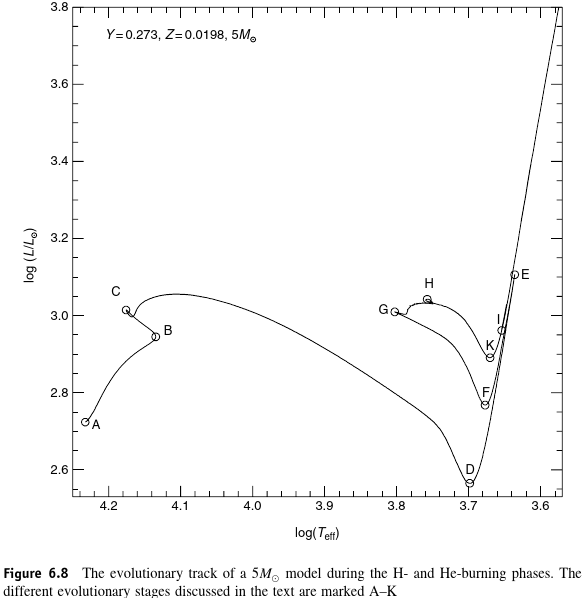
\includegraphics[trim={0cm 0cm 1cm 0cm},clip, keepaspectratio,height=0.4\textheight]{5MtoHB}\label{fig:5MtoHB}
	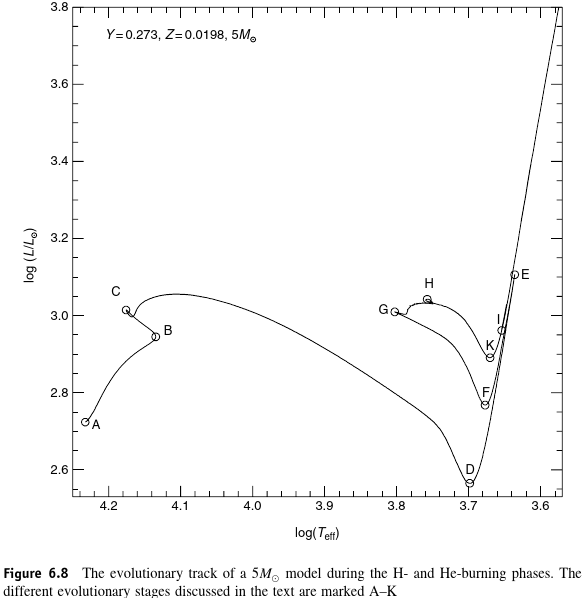
\includegraphics[trim={0cm 0cm 1cm 0cm},clip, keepaspectratio,height=0.4\textheight]{5MtoHB}\label{fig:5MtoHB}
	\end{figure}
\end{column}\end{columns}
\end{frame}

\begin{frame}{Deps of blue loop on params}
	\begin{itemize}
	\item Morphology of BL have non-linear dep on params [160]
	\item $M<10-12\msun$ B-loop increases with M, for more massive stars He ignites before Hayashi track - blue loop disappears
	\item extension B-loop increases, \xaumenta{Y}, decreases, \xdiminuisce{Z}
	\item B-loop seems favoured by sharper H profile in envelope (changes in H-burning efficiency as shell encounter discontinuity): CE overshoot produce enhanced discontinuity during dredge-up I: deeper convective envelope reaches regions more He-rich produced in MS
	\item increasing efficiency of overshoot of CC overshoot during H-burning strongly reduces B-loop extension
	\item If H-burning shell encounters chem. disc. before He-core ignition overshoot has no effect on B-loop
	\item Envelope overshoot may be able to trigger a B-loop: enhanced discontinuity during first dredge-up - deeper convective envelope reaches regions with more He produced in MS
	\item Increase of CC overshoot during H burning strongly reduces extension of B-loop
\end{itemize}
\end{frame}

\subsection{Pulsations of He-core burning stars}\linkdest{HBpulsating}

\begin{frame}{instability strip (cepheid IS)}
%Refs: [61], [79], [80]
\begin{columns}[T]
	\begin{column}{0.55\textwidth}
	\begin{itemize}
	\item stable radial pulsation: $\kappa$-mechanism - star energy flow fixes the radius - stability implies variation in energy flux and thus in R - opacity increases during compression/decreases in expansionat same level in stellar envelope: He/H ionization ragions
	Boundary of IS - cool boundary: \xdiminuisce{T_e}, convection set in - hot boundary: \xaumenta{T_e}, \xdiminuisce{M_{ion}}, \xaumenta{R_{ion}}
	\item RR Lyrae and classic cepheids: \keyword{Standard candles} for PopI/II stars
	\item Adiabatic pulsation with period $\Pi\sqrt{\rho}=Q$, slightly deps on M: $\Pi\propto	\sqrt{\frac{R}{g_s}}\propto\sqrt{\frac{R^3}{M}}$ 
	\end{itemize}
	\end{column}
	\begin{column}{0.45\textwidth}
	\begin{figure}[!ht]
	%\includegraphics[trim={0cm 0cm 1cm 0cm},clip, keepaspectratio,height=0.37\textheight]{ffiig}\label{fig:ffiigg}
	\end{figure}
\end{column}\end{columns}
\end{frame}

\begin{frame}{RR Lyrae stars: low mass stars crossing IS during He-core burning}
\begin{columns}[T]
	\begin{column}{0.55\textwidth}
		\begin{itemize}
			\item He ionization region is $\num{e-7}\msun$, R varies by $20\%$, L by factor 2, $\Pi\approx0.2-0.9\si{\day}$ amplitude \SIrange{0.2}{1.6}{\mag} in B-band - ab-type fundamental tone (asymmetric), c-type (symmetric) first overtone,
		\end{itemize}
	\end{column}
	\begin{column}{0.45\textwidth}
	\begin{figure}[!ht]
	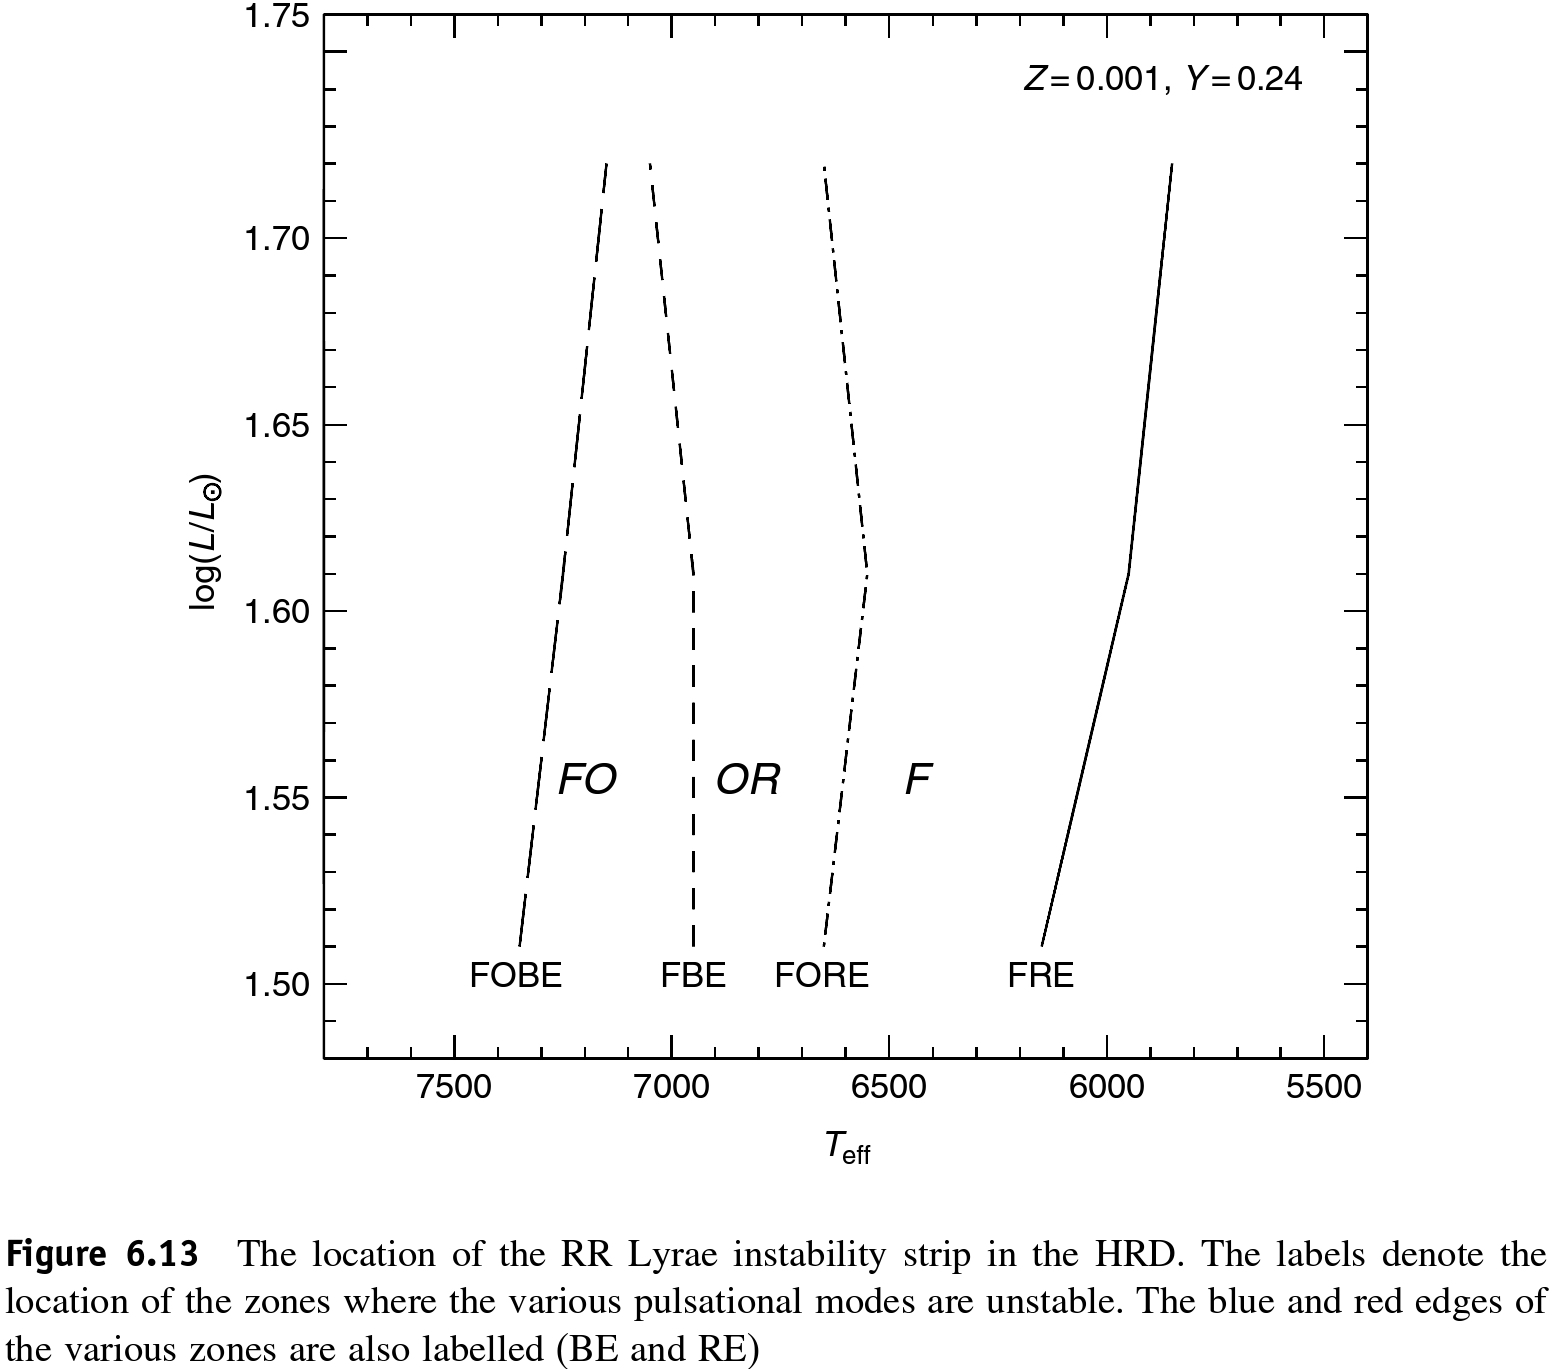
\includegraphics[trim={0cm 0cm 1cm 0cm},clip, keepaspectratio,height=0.45\textheight]{HBPulsation-RRIS}\label{fig:HBPulsation-RRIS}
	\end{figure}
\end{column}\end{columns}
connection between $\Pi$ and other stellar parameter for ab-stars ([16]):
\begin{align*}
&\log{\Pi}=11.627+0.823\log(\frac{L}{\lsun})-0.582\log(\frac{M}{\msun})-3.506\log(T_e)\\
&=11.627+0.823A-3.506\log(T_e)
\end{align*}
L of HB stars is strongly deps on Y ([35]): relation between $\Pi/A$ is usefull to infer $He_{in}$
\end{frame}

\begin{frame}{RR-Lyrae stars: Bailey and Petersen diagrams}
\begin{columns}[T]
\begin{column}{0.55\textwidth}
	\begin{itemize}
	\item Petersen diagram: $\Pi_1/\Pi_0$ vs $\Pi_0$
	\item Bailey diagram: Comparison of theoretical/empirical result for amplitude vs $\Pi$
	\end{itemize}
	\end{column}
	\begin{column}{0.45\textwidth}
	\begin{figure}[!ht]
	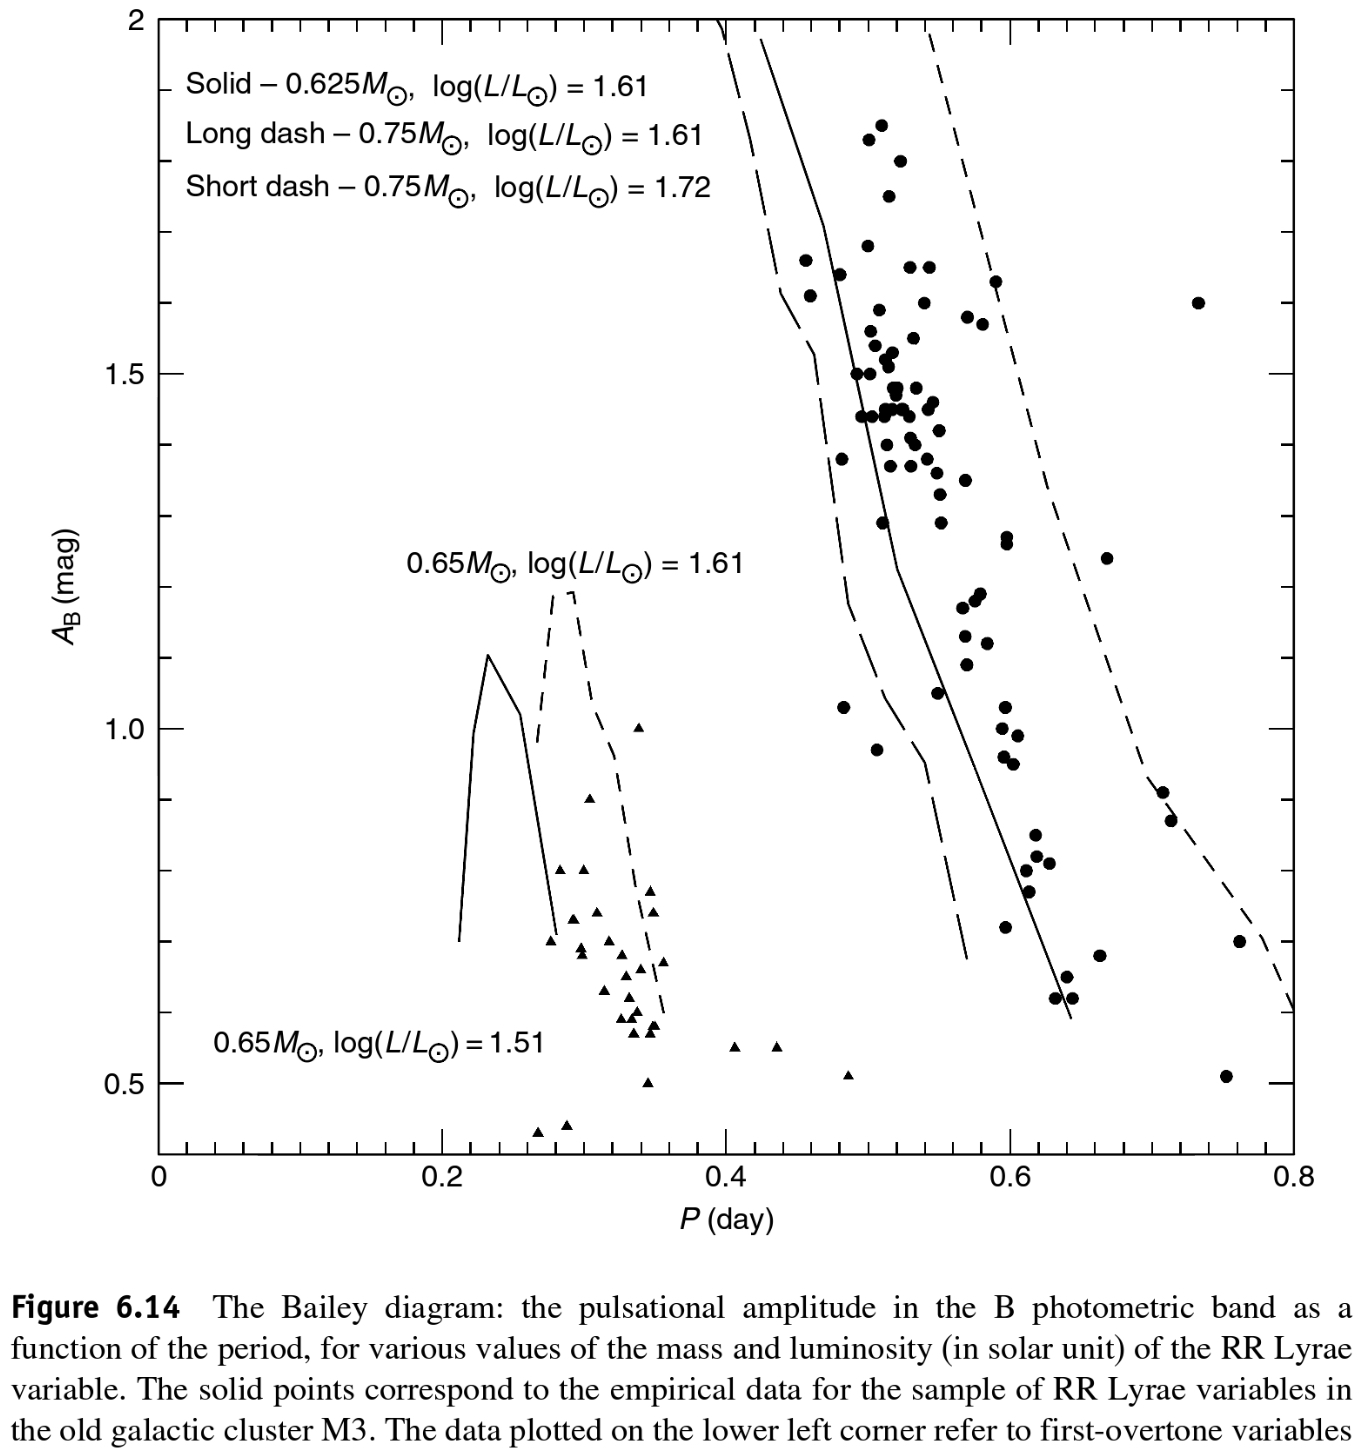
\includegraphics[trim={0cm 0cm 1cm 0cm},clip, keepaspectratio,height=0.37\textheight]{HBPulsating-B}\label{fig:HBPulsating-B}
	\end{figure}
\end{column}\end{columns}
\end{frame}

\begin{frame}{classic Cepheids: Int-mass stars going through He-burning with B-loop extends to IS}
\begin{columns}[T]
	\begin{column}{0.55\textwidth}
		\begin{itemize}
			\item $L\approx300-2500\lsun$, $\Pi\approx1-50\si{\day}$
			\item P-L relation: scale-distance of universe
			\item Topology of cepheids IS is very diff from RR-Lyrae ([18])
			\item \xaumenta{Z}, \xdiminuisce{T_e}, steeper IS
		\end{itemize}
	\end{column}
	\begin{column}{0.45\textwidth}
		\begin{figure}[!ht]
			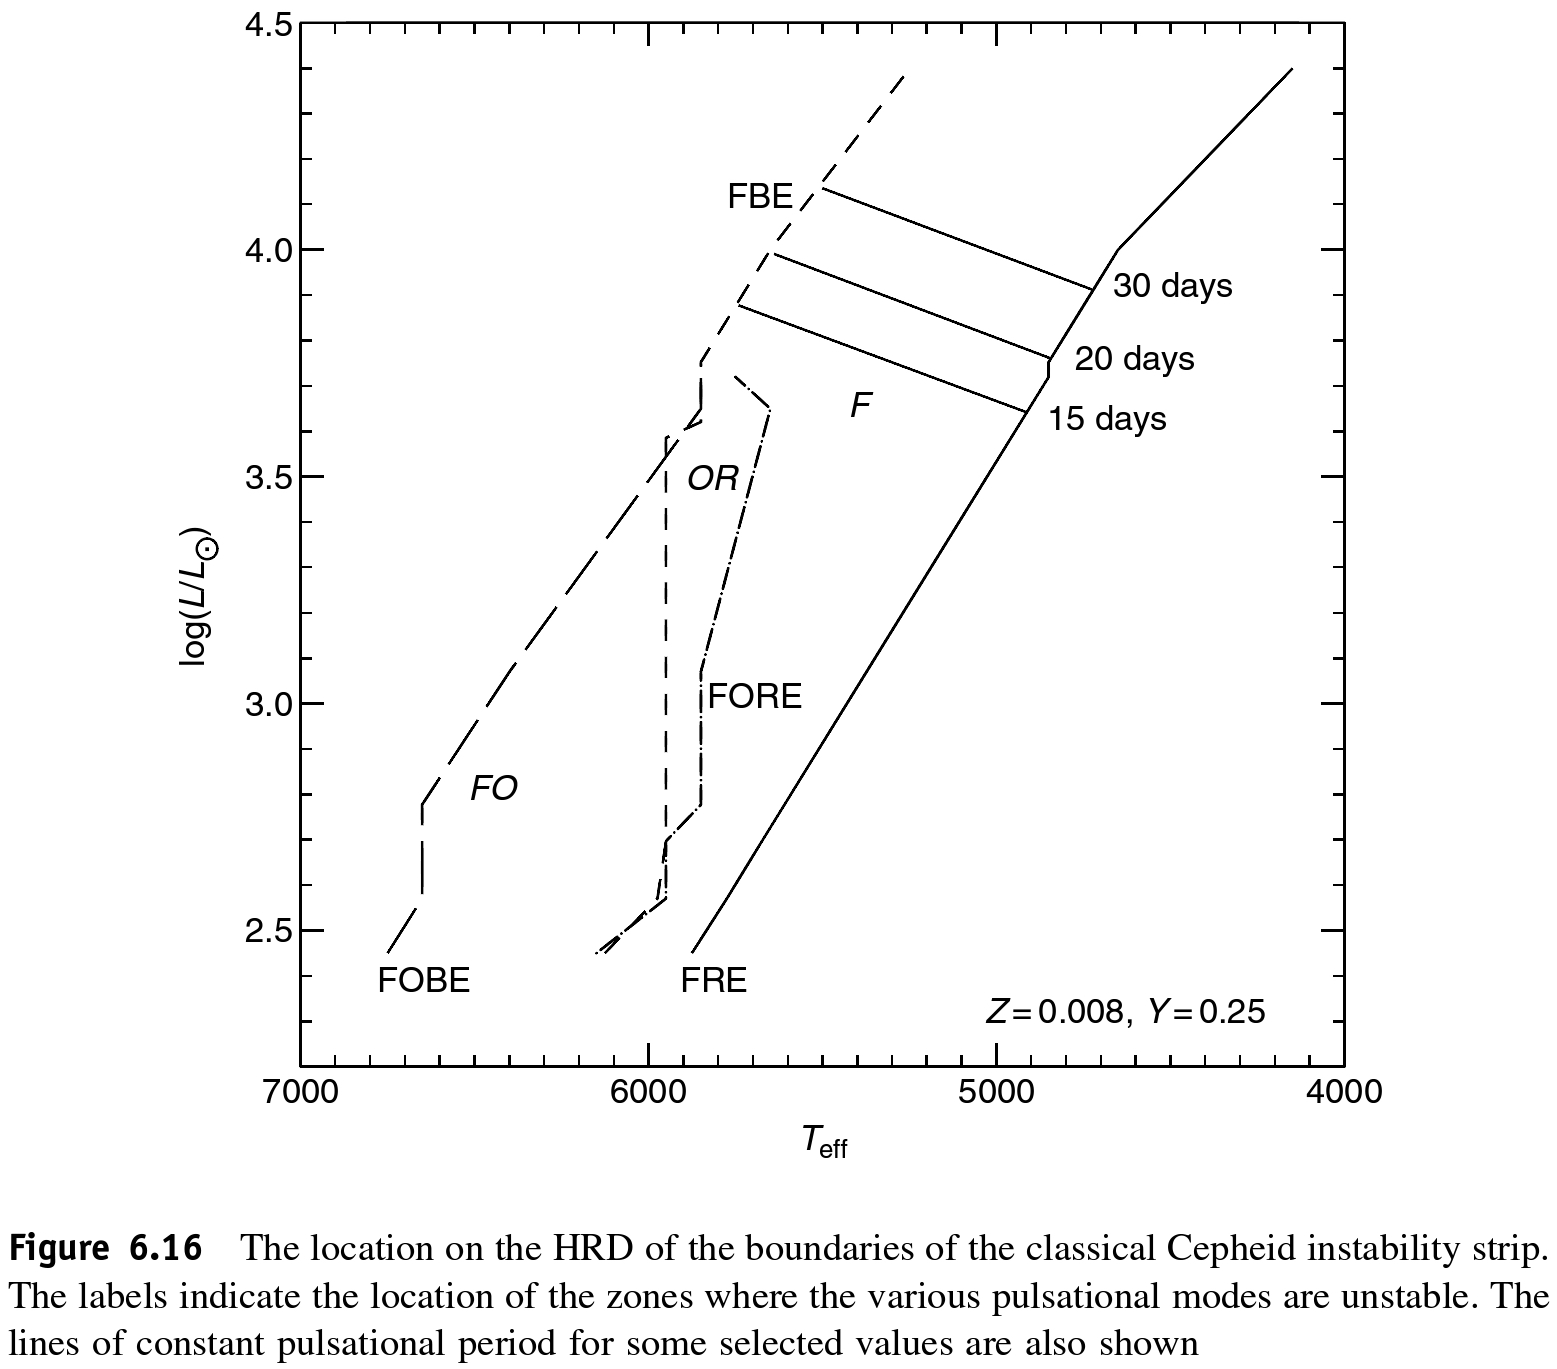
\includegraphics[trim={0cm 0cm 1cm 0cm},clip, keepaspectratio,height=0.4\textheight]{HB-cCIS}\label{fig:HB-cCIS}
		\end{figure}
\end{column}\end{columns}
For solar composition and $\Pi_0$:
\begin{align*}
&\log{\Pi}=0.987-3.108\log{T_e}-0.767\log{\frac{M}{\msun}}+0.942\log{\frac{L}{\lsun}}\\
&\exv{M_A}=a+b\log{\Pi}+c(CI)
\end{align*}
CI=color index. Tight relation between mass and surface luminosity of stars at beginning of He-core burning
\end{frame}

\subsection{Ramo asintotico (AGB)}\linkdest{AGB}

\begin{frame}{Index - Evoluzione in AGB}
Ingresso in agb: clump. AGB manqu\'e. Secondo Dredge-up; pulsi termici; terzo dredge-up
\end{frame}

\begin{frame}{Evoluzione in AGB: EAGB}
\begin{columns}[T]
	\begin{column}{0.55\textwidth}
	\begin{itemize}
	\item End of He-burning: He-core becomes low enough star move in HDR toward lower $T_e$/ larger $L$ (Asymptotic for $M_*<2.5\msun$): $T_e-L$ relationship similar to RGB (Hayashi track).
	\item Early AGB: He-burning shift to shell moving outward in He-core around CO-core of increasing mass due to $He\to C/O$ in shell; H-burning shell is turned off due to expansion caused by He-burning shell (T drops)
	\item \keyword{AGB clump}: in low $M_*$ onset of He-burning shell causes H-shell to switch off: \xdiminuisce{L_s} per ri-aumentare as \xaumenta{M_c} - stars cross 3-times same HDR region - well populated old galactic stellar system
	\end{itemize}
	\end{column}
	\begin{column}{0.45\textwidth}
	\begin{figure}[!ht]
	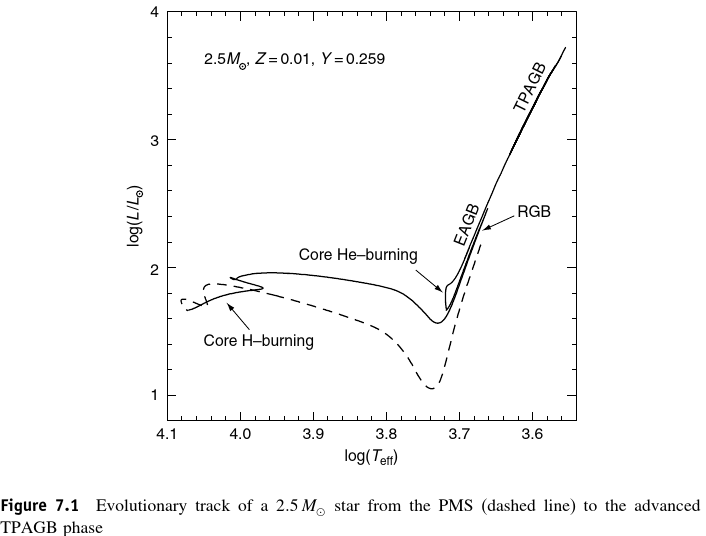
\includegraphics[trim={0cm 0cm 1cm 0cm},clip, keepaspectratio,height=0.4\textheight]{PMS2AGB-lowM}\label{fig:PMS2AGB-lowM}
	\end{figure}
\keyword{Early AGB} and \keyword{second dredge-up}: for $M_*>3-5\msun$ expansion of layers above and cooling let the outer convection penetrate H-depleted zone: up $1\msun$ of dredged-up material ($He$, $^{12}C$, $^{16}O\to^{14}N$); reduction of H-depleted region prevent formation of massive WD
\end{column}\end{columns}
\end{frame}

\begin{frame}{CO-core state at end of HE-burning}
\begin{itemize}
\item Plasma neutrino loss: $M_*<8-10\msun$ compact CO-core with $\rho_C\approx\SIrange{e5}{e8}{\gram\per\cubic\cm}$ highly degenerate - plasma neutrino loss is balanced by contraction and cooling: cooling is max at center - $T_M$ moves outward
\item Limit mass $M_{up}$ where \Pelectron degeneracy prevent CO-core ignition: depends strongly on initial composition - for solar composition $M_{up}\approx8\msun$, has minimum for $Z\approx0.001$ at $M_{up}\approx4\msun$
\item $M_*>M_{up}$: CO-core ignites (quitely/flash)
\end{itemize}
\end{frame}

\begin{frame}{Thermally Pulsating AGB phase}
\begin{columns}[T]
	\begin{column}{0.48\textwidth}
 	When He-burning shell encounters H/He discontinuity dies - after rapid contraction H-burning shell provide star's energy needs - He ashes accreted on CO-core are compressed/heated until a critical mass is reached - $\approx\num{e-3}\msun$ for $0.8\msun$ CO-core - He ignited in runaway manner due to geometrical thickness of the shell - $L_{peak}\approx\numrange{e7}{e8}\lsun$.
	H-burning shell is turned of by expansion/cooling due to He-Burning - convective envelope from He-burning shell up to H/He discontinuity
	\end{column}
	\begin{column}{0.52\textwidth}
		\begin{figure}[!ht]
			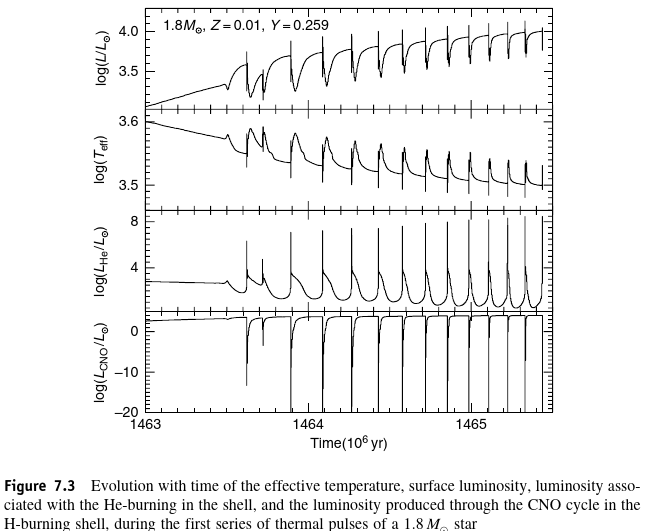
\includegraphics[trim={0cm 0cm 1cm 0cm},clip, keepaspectratio,height=0.38\textheight]{TPAGB-LTe}\label{fig:TPAGB-LTe}
		\end{figure}
	As \xdiminuisce{\epsilon_{He}} \xdiminuisce{L_{He}}: for $M_c>0.7\msun$ decrese in L causes convective shell to disappear - for lower mass convection extends to incomplete He-burning regions: steady state nuclear burning and energy outflow.
\end{column}\end{columns}
After all product of H-shell is burnt H-burning shell turn on again (many repetition): pulse amplitude grows to asymptotic regime: $\epsilon_H$ depends on mass of He-core - $M_{cHe}-L_s$ relationship (as in RGB)
\end{frame}

\begin{frame}{\keyword{Properties of burning shell}}
Refs: [115], [155] - In a shell of thickness s located at r:
\begin{columns}[T]\begin{column}{0.5\textwidth}
\begin{align*}
&\frac{dP}{P}=4\frac{s}{r}\frac{d\rho}{\rho}\\
&(4\frac{s}{r}-\alpha)\frac{d\rho}{\rho}=\beta\frac{dT}{T}
\end{align*}
\end{column}
\begin{column}{0.5\textwidth}
\begin{align*}
&\frac{dP}{P}=\alpha\frac{d\rho}{\rho}+\beta\frac{dT}{T}
\end{align*} 
\end{column}\end{columns}
Stable burning requires $4\frac{s}{r}>\alpha$ so if shell is too shallow an expansion causes \xdiminuisce{\rho} e \xaumenta{T}.
\end{frame}

\begin{frame}{Convective phenomena during TPAGB}
\begin{columns}[T]
\begin{column}{0.55\textwidth}
\begin{itemize}
\item After He-shell reignition convective envelope can move inward and cross H/He discontinuity: during \keyword{Dredge-up III} He-burning product/s-elements are dredged-up to surface (\keyword{C-star}: $O/C\ll1$ in photosphere) - \xaumenta{M_{DU}} as \xaumenta{M_C}, after maximum, \xdiminuisce{M_{DU}} as \xdiminuisce{M_e} - \xdiminuisce{Z}, DUIII penetrates deeper (diff sufrace abundance galactic AGB-Z poor AGB)
\item Convection penetrates deeper when pulse is stronger (more expansion/cooling): determined by thermal condition at bottom of He-rich layers - \xdiminuisce{\epsilon_H} maggiore \'e la densit\'a sul fondo di He-shell stronger TP - $\epsilon_H$ deps on $M_e$ (wind, burnt), H-exhausted region mass, chem-comp
\end{itemize}
\end{column}
\begin{column}{0.45\textwidth}
\begin{figure}[!ht]
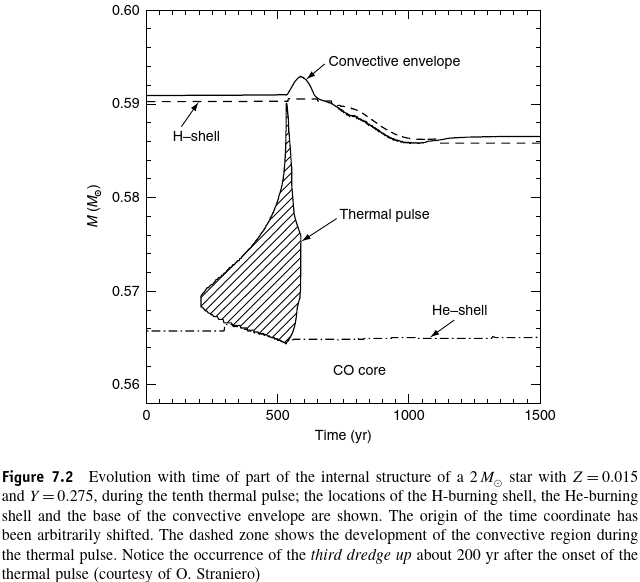
\includegraphics[trim={0cm 0cm 1cm 0cm},clip, keepaspectratio,width=0.99\textwidth]{TPAGB-3DU}\label{fig:TPAGB-3DU}
\end{figure}
Minimum for DUIII $M_e\approx0.4\msun$: $M_{ZAMS}<1.4-1.5\msun$ don't have DUIII - we don't expect C-rich stars in old pop
\end{column}\end{columns}
\end{frame}

\begin{frame}{Nucleosintesi in AGB: s-elements}
\begin{columns}[T]
\begin{column}{0.55\textwidth}
\begin{itemize}
\item Spectroscopical obs: AGB surface enriched of \keyword{s-elements} (Sr, Y, Zr, Ba, La, Ce, Pr, Nd) produced via ''slow'' neutron capture - $^{99}Tc$ on surface $\tau\approx\SI{2e5}{\year}$ prove it's not pollution due to accretion of primeval material
\item During first inter-shell mixing N(circa 5 volte l'abbondanza di elementi CNO iniziale) $^{14}N\to^{22}Ne$
\item if at TP at base of intershell $T>\SI{3.5e8}{\kelvin}$ first neutron production reaction take place as in int-M AGB ([103]), for $M_*<3\msun$ $T>\SI{9e7}{\kelvin}$ for second reaction
\end{itemize}
\end{column}
\begin{column}{0.45\textwidth}
n production ([30,32]):
\begin{align*}
&^{22}Ne(\alpha,n)^{25}Mg\\
&^{13}C(\alpha,n)^{16}O
\end{align*}
[208]: 2nd fully burn in rad region between 2P (\num{e7} n). Rimozione di N (which capture n) da inter-shell:
\begin{align*}
&^{14}N(\alpha,\gamma)^{18}F(\beta^+,\nu)^{18}O(\alpha,\gamma)^{22}Ne
\end{align*}
Produzione/distruzione di $^{13}C$
\begin{align*}
&^{12}C(H,\gamma)^{13}N(\beta^+,\nu)^{13}C\\
&^{13}C(H,\gamma)^{14}N
\end{align*}
\end{column}\end{columns}
\keyword{Tasca di $^{13}C$}: In inter-shell after convective episode is present $^{12}C$ but not $^{14}N$ - $^{13}C$ can be produced if right amount of H (diffusion, overshoot, rotational mixing, gravity waves) - [104]: after DUIII (\keyword{post-flash dip}) sharp disc. between H-rich env/He-/C-rich intershell until H-reignition (\SI{e4}{\year}) and then heated up form $^{13}C$
\end{frame}

\begin{frame}{Hot-bottom burning ([209])}
$M_*>6-7\msun$ at base of convective zone ($T\approx\SI{8e7}{\kelvin}$) happens significant burn: \xaumenta{L_s} (breaks of $M_c-L$ relation) - s composition is strongly affected: $C\to N$, Li production through \keyword{Cameron-Fowler mechanism} [33] - when envelope has $T\approx\SI{e8}{\kelvin}$ $^3He+^4He\to^7Be+\gamma$ very efficiently then $^7Be+\Pelectron\to^7Li+\Pnue$: $^7Li$ can survive $T<\SI{2.5e6}{\kelvin}$. Amount of surface-Li after envelope retreats is determined by balance of $^7Be$ transported toward surface and Li produced at $T<T_b$ transported inside. [231]: Brightest long period variables (TPAGP experiencing large amplitude pulsation) are super-Li object (3 O.M. then expected)
\end{frame}

\begin{frame}{AGB termination}
\begin{columns}[T]
	\begin{column}{0.6\textwidth}
	\begin{itemize}
	\item $M_*>1.4\msun$ (Chandrasekhar limit): C-ignition, AGB ends - we don't expect $M_{CO}$ becomes suff. larger during TPAGB (mass loss)
	\item When $M_e<\num{e-3}\msun$, $\epsilon_H\to0$, \xaumenta{T_e} - \keyword{superwind} terminate AGB phase - brightest AGB in different systems show same luminosity: mass loss strongly increases at AGB's end ($\num{e-4}\msun\si{\per\year}$)
	\item Evolution of low mass star: TPAGB to WD - once $M_e$ below critical limit star move \xaumenta{T_e} at constant L - burning H in thin shell until bluest point then both H-/He-rich envelope contracts rapidly. Thermal envelope conditions determine which: i) nuclear burning dies (WD) ii) Heating He-shell burn-again AGB (runaway He-burning then quite):
	\end{itemize}
	\end{column}
	\begin{column}{0.4\textwidth}
\begin{figure}[!ht]
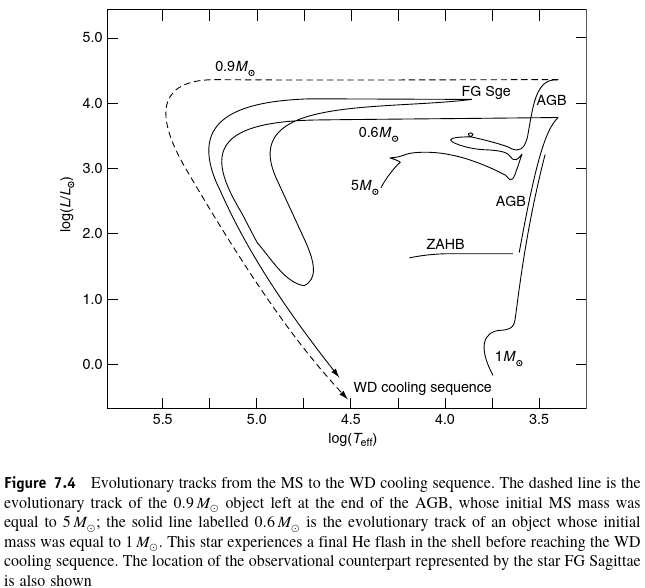
\includegraphics[trim={0cm 0cm 1cm 0cm},clip, keepaspectratio,width=0.99\textwidth]{lateevol-MS2WD}\label{fig:lateevol-MS2WD}
\end{figure}
star evolve to blue side (FG-sagittae) with timescale 3 times that of H-shell burning. iii) Heating-burning of H envelope in runaway manner: \keyword{selfinduced nova}/\keyword{planetary nebula}
\end{column}\end{columns}
\end{frame}

\begin{frame}{Pulsating AGB stars: Empirical Mass loss-Period relation}
\keyword{Mira-variable star}: during AGB stars have large amplitude pulsation - Strong correlation between pulsation and mass loss: compression favour molecules/grains formation (Radiation-driven mass loss: $\numrange{e-8}{e-4}\msun\si{\per\year}$)
Empirical mass loss-$\Pi$ relation:
\begin{align*}
&\Pi<500[\si{\day}]:\\
&\log(\TDy{t}{M})\approx-11.4+0.0123\log(\Pi)\\
&\Pi>500[\si{\day}]:\\
&\TDy{t}{M}\approx\num{6.07023e-3}\frac{L}{cv_e}
\end{align*}
\end{frame}

\begin{frame}{AGB termination:Self-induced novae-Planetary nebulae}
\begin{itemize}
\item a) violent ejection H-rich envelope: WD without H on surface (non DA/DB WD), b) After quite H-burning cools down to WD: non-DA (wind).
\item After super-wind the ejecta of TPAGB composition keep expanding - when $T_e\geq\SI{3e4}{\kelvin}$ are ionized: assume characteristics and shape of PN
\end{itemize}
\end{frame}

\subsection{Evoluzione in nane bianche e evoluzione di stelle massicce}\linkdest{WD-intmM}

\begin{frame}{Chandrasekhar limit-mass e CO-core close to $M_{up}$}
$M_{Ch}$ upper mass limit for fully relativistic degenerate core in HE [59] - $M_*>M_{up}$ don't develop degenerate CO-core
\begin{columns}[T]
\begin{column}{0.4\textwidth}
\begin{block}{Equazione di stato elettroni degeneri}
\begin{align*}
&P_e=K_{NR}(\frac{\rho}{\mu_e})\expy{\frac{5}{3}}\\
&P_e=K_R(\frac{\rho}{\mu_e})\expy{\frac{4}{3}}
\end{align*}
\end{block}
\begin{block}{Massa limite per CO-core}
Per CO-core $\mu_e=\approx2$ ($n_e=\frac{\rho}{\mu_em_H}$, $\invers{\mu_e}=\sum\frac{X_iZ_i}{A_i}$)
\begin{align*}
&M_{Ch}=1.459(\frac{2}{\mu_e})^2\msun=1.46\msun
\end{align*}
\end{block}
\end{column}
\begin{column}{0.6\textwidth}
\begin{itemize}
\item No WD observed near $M_{Ch}$
\item WD most commond end of stellar evolution ($95\%$ of galaxy's stars)
\item Evolution of CO-core similar to degenerate He-core in RGB for low-$M_*$
\item Prop of CO-core unaffected by envelope as long as has not enough mass to nuclear burning
\item \xaumenta{M_{CO}}, \xaumenta{\rho_c} as He-burning in shell [pg 89']: flusso di plasma neutrini dalla parte centrale \xaumenta{\epsilon_{\nu}}(segno meno nel energy equation) - $\epsilon_C\to\epsilon_{\nu}$ per $M_*\to M_{Ch}$
\item \xaumenta{M_{CO}} \xaumenta{\epsilon_C} - Explosive CO-burning: \keyword{SN-I-1/2}

\end{itemize}
\end{column}
\end{columns}
\end{frame}

\begin{frame}{Caratteristiche WD}
\begin{columns}[T]
	\begin{column}{0.61\textwidth}
		\begin{itemize}
		\item $\exv{M}_WD\approx\numrange{0.55}{0.6}\msun$, faintest $L\approx\num{e-4.5}\msun$, $\frac{R}{\rsun}\approx0.01(\frac{\msun}{M})\expy{1/3}$: large $\exv{\rho}$, $\large{g_s}$, low $L_s$
		\item Uncertainty in progenitor mass is due to uncertainty in mass loss
		\item M-R rel: $P_c\approx P_e$ NR-deg - $\frac{M\expy{5/3}}{R^5\mu_e\expy{5/3}}\propto\frac{GM^2}{R^4}$ quindi $R\propto\frac{1}{G\mu_e\expy{5/3}}M\expy{-1/3}$
		\item \xaumenta{M_{WD}}, \xaumenta{\tau_{cool}}: per $L\approx\num{e-3}\lsun$ $\tau_{cool}\approx\SI{e9}{\year}$
		\item He-WD: RGB stars that have lost envelope (mass loss, mass transfer) - $M_{WD}\approx\numrange{0.15}{0.5}\msun$ - brighter at fixed age as \xdiminuisce{\mu}
		\item O-Ne WD endpoint of $M_*\approx8-11\msun$ at end of C-burning ($M_{WD}^{ONe}\approx\numrange{1}{1.2}\msun$)[78] - shorter cooling due to \xaumenta{\mu}; cryst. at higher T [91]
		\end{itemize}
	\end{column}
	\begin{column}{0.39\textwidth}
		\begin{figure}[!ht]
			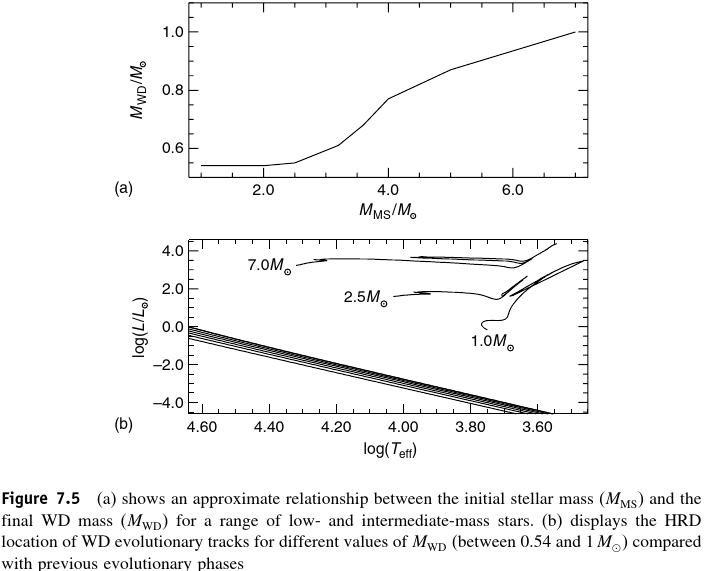
\includegraphics[trim={0cm 0cm 1cm 0cm},clip, keepaspectratio,height=0.38\textheight]{WD-ML}\label{fig:WD-ML}
			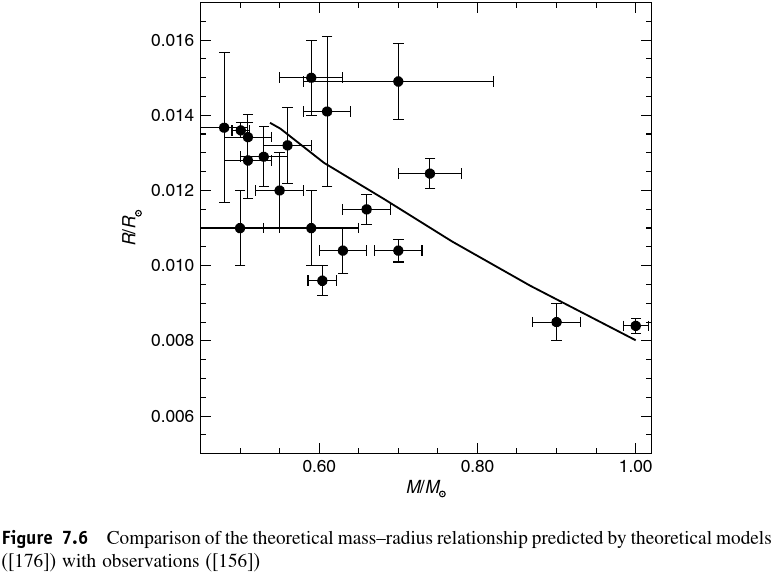
\includegraphics[trim={0cm 0cm 1cm 0cm},clip, keepaspectratio,height=0.38\textheight]{WD-MR}\label{fig:WD-MR}
		\end{figure}
\end{column}\end{columns}
\end{frame}

\begin{frame}{Simplified WD model: $L-T_c$ relation and envelope size}
\begin{block}{$L-T_c$ relation}
m-continuity + HE - $\frac{M}{R^3}\propto\exv{\rho}$ - considering radiative envelope: $\frac{HE}{RT}=P\,dP=\frac{4ac}{3}\frac{4\pi GMk}{\kappa_0L\mu m_H}T\expy{7.5}\,dT$ (EOS: perfect gas, opacity: $\kappa=\kappa_0\rho T\expy{-3.5}$, $m_r\approx M$) - integrating from surface we have enevelope $P(T)$ and via EOS: $\rho=\sqrt{\frac{32\pi acGM\mu_{env}m_H}{8.5*3\kappa_0Lk}}T\expy{3.25}$ - at envelope/degenerate boundary $P_e^d=P_e^{perf}$: $\frac{\rho_bkT_b}{\mu_em_H}=\num{1.0036e13}(\frac{\rho_b}{\mu_e})\expy{5/3}$ (cgs) quindi $\frac{L}{\lsun}=\num{6.4e-3}\frac{\mu}{\mu_e}\frac{M}{\msun}\frac{T_b\expy{3.5}}{\kappa_0}$. CO WD deg.-core is isothermal $T_b\approx T_c$ - $L\approx\numrange{e-3}{e-4}\lsun$ so $T_c<\SI{e7}{\kelvin}$ - detailed $L-T_c$ relation [177]
\end{block}
\begin{block}{Envelope size}
Rad+Kramers - $\TDy{r}{T}=-\frac{3\kappa_0\rho^2}{4acT\expy{6.5}}\frac{L}{4\pi r^2}$ -+above $\rho$: $\frac{dr}{r^2}=4.25\frac{k}{\mu Gm_H}\frac{dT}{M}$ - Integrata da s a $r_b$: $T_b=\frac{1}{4.25}\frac{\mu Gm_H}{k}\frac{M}{R}(\frac{R}{r_b}-1)$ - $T_b\approx\SIrange{e6}{e7}{\kelvin}$ cio\'e $r_b\approx0.99R$
\end{block}
\end{frame}

\begin{frame}{Simplified WD model: Cooling law - legge di Mestel}
Luminosity is equals rate of decrease of thermal energy of ions - in e-deg core $C_VT=\frac{3}{2}kT$ per ion/ total thermal energy $E_i=\frac{3}{2}kT\frac{M}{\mu_im_H}$ ($\frac{M}{\mu_im_H}$ total number of ions in core) - $T\approx\SI{e7}{\kelvin}$, $E_i\approx\SI{e48}{\erg}$:
\begin{align*}
&L=-\TDy{t}{E_i}=\alpha MT\expy{7/2}\ \Rightarrow\ \alpha T\expy{7/2}=-\TDy{t}{T}\frac{3k}{2\mu_im_H}\\
&t-t_0=\frac{3k}{5\alpha\mu_im_H}(T\expy{-5/2}-T_0\expy{-5/2})
\end{align*}
when $T_0\gg T$: $\Delta t=t-t_0=\approx\frac{3kT\expy{-5/2}}{5\alpha\mu_im_H}$ quindi \keyword{Legge di Mestel}:
\begin{equation*}
\Delta t[\si{\year}]\propto(\frac{L}{M})\expy{-5/7}\approx\frac{\num{4.5e7}}{\mu_i}(\frac{L\msun}{M\lsun})\expy{-5/7}
\end{equation*}
Effects not included in Mestel law: i) Crystallinization ii) Envelope: possible H-burning, opacity evolution as degenerate core cools causes convective instability in envelope, contribute to energy budget by slow contraction
\end{frame}

\begin{frame}{Crystallization}
\begin{columns}[T]
	\begin{column}{0.5\textwidth}
ion phase transition: liquid phase for $1<\Gamma<180$ and solid phase for $\Gamma>180$ - correction due to coulomb interaction, oscillation around lattice equilibrium position and quantum correction $\theta=\frac{\theta_D}{T}>1$ (\keyword{Debye temperature}: $\theta_D=\num{4e3}\rho\expy{1/2}\si{\kelvin}$). $c_v\approx\frac{3}{2}K$ per $\Gamma<1$, as \xdiminuisce{T} \xaumenta{\Gamma} and \xaumenta{c_v} until maximum at $\Gamma\approx180$ then decreases from $T\approx\theta_D$ as $c_v\propto T^3$
	\end{column}
	\begin{column}{0.5\textwidth}
	\begin{figure}[!ht]
	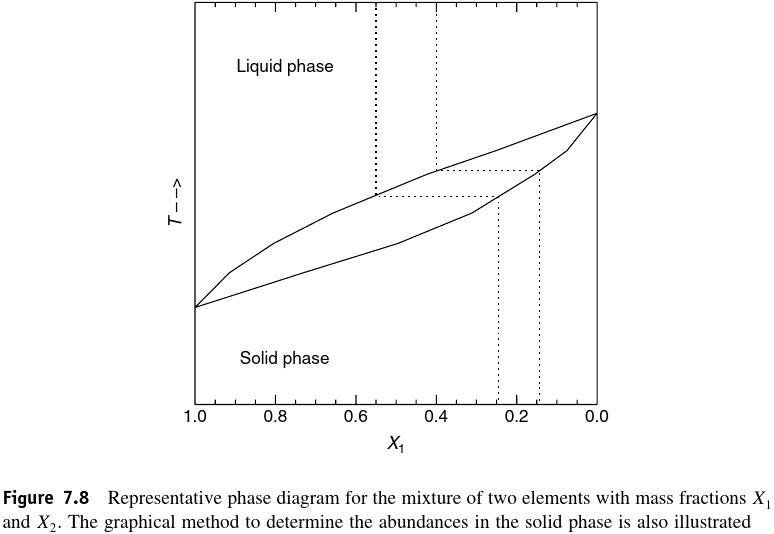
\includegraphics[trim={0cm 0cm 1cm 0cm},clip, keepaspectratio,height=0.4\textheight]{WD-phasetransition}\label{fig:WD-phasetransition}
	\end{figure}
\end{column}\end{columns}
Free-energy: ideal eos (no coulomb $C_V=\frac{3}{2}k$) + correction $F_C$
\begin{align*}
&F_C=NkT(-0.89752\Gamma+3.78176\Gamma\expy{1/4}-0.71816\Gamma\expy{-1/4}\\
&+2.19951\ln\Gamma-3.30108)\tag*{liquid}\\
&F_C=NkT(-4.29706+4.5\ln\Gamma-\frac{1490}{\Gamma^2})\tag*{solid}
\end{align*}
\end{frame}

\begin{frame}{detailed computation: phase transition latent heat}
\begin{columns}[T]
	\begin{column}{0.5\textwidth}
		\begin{itemize}
		\item Cr. start for $1\msun$ at $\log(\frac{L}{\lsun})\approx-2.7$ and reaches boundary of deg core at $\log(\frac{L}{\lsun})\approx-4.2$: \xdiminuisce{M_{WD}} crystallization start at lower L (lower $T_c$) as \xdiminuisce{\rho_c} $\Gamma\approx180$ when they are cooler
		\end{itemize}
	\end{column}
	\begin{column}{0.5\textwidth}
		\begin{figure}[!ht]
		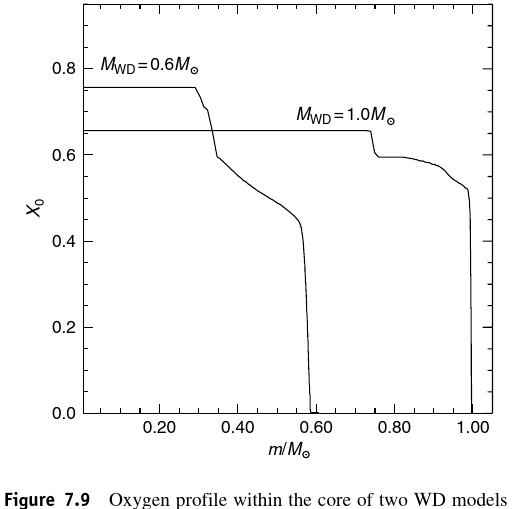
\includegraphics[trim={0cm 0cm 1cm 0cm},clip, keepaspectratio,height=0.4\textheight]{WD-Xopostcry}\label{fig:WD-Xopostcry}
		\end{figure}
	\end{column}\end{columns}
\end{frame}

\begin{frame}{detailed computation: cooling law}
\begin{columns}[T]
	\begin{column}{0.5\textwidth}
		\begin{itemize}
			\item $\rho$ higher in center so crystallization front move outward as $\Gamma\geq180$: release latent heat $q\approx kT$ (difference in S between phases) per ion (cooling slow down resp to M-law)
			\item earlier cryst. shorter cooling delay: $\Delta t\approx\frac{\Delta E}{L}$ ($\Delta E$ injected at cryst.)
		\end{itemize}
	\end{column}
	\begin{column}{0.5\textwidth}
		\begin{figure}[!ht]
			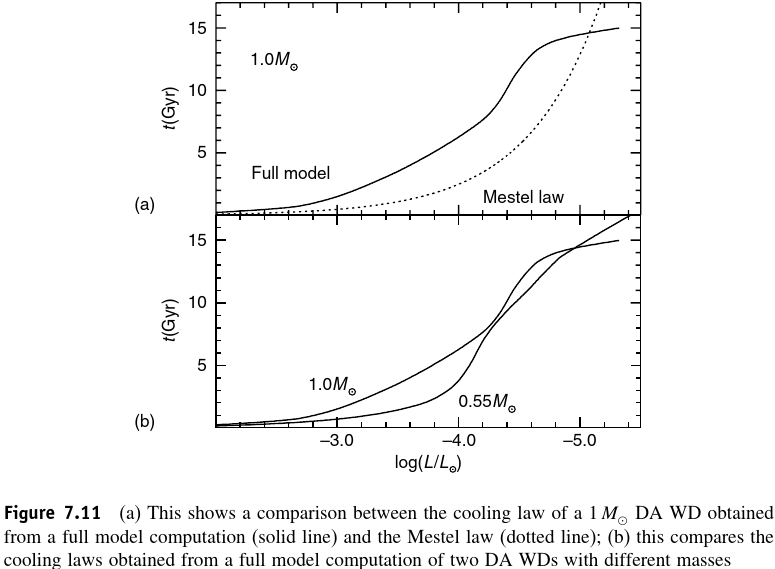
\includegraphics[trim={0cm 0cm 1cm 0cm},clip, keepaspectratio,height=0.4\textheight]{WD-coolingMvsfm}\label{fig:WD-coolingMvsfm}
		\end{figure}
\end{column}\end{columns}
Hot WD: faster cooling then M-law ($L_S+L_{\nu}$) -when $\log(\frac{L}{\lsun})\leq-1.0$ cooling slow down and becomes longer slow envelope contraction and \xaumenta{c_v} until $\theta_D$ in core - \xaumenta{M_{WD}}, \xaumenta{\tau_{cool}},core reaches $\theta_D$ at higher luminosity \xdiminuisce{\tau_{cool}} shorter then M-law at low L
\end{frame}


\begin{frame}{detailed computation: chem separation [77,107]}
\begin{columns}[T]
	\begin{column}{0.65\textwidth}
		\begin{itemize}
			\item given ratio $\frac{X_C}{X_O}$ CO mixture in gas/liquid phase at cryst. can't be mainteined due to not fully miscibility in solid phase - suppose $X_1<X_2$ as in central regions of CO core and that phase diagram told us that $X_1$ in crystallized phase is lowered then at liquid-cryst boundary $X_1$ increased quindi \xdiminuisce{\mu} in above layers e si ha instabilit\'a convettiva and mixing with above layers so final profile isn't homogeneous
			\item changes of $\mu$: $\epsilon_g=\TDy{\mu}{U}|_{T,V}\TDy{t}{\mu}$ - \xaumenta{\tau_{cool}}($10\%$)
			\item At end of AGB: O-profile flat until end of convective He-core, bump outside due to He-burning shell crossing semiconvective CO-enriched regions ($^{12}C+\alpha\to^{16}O+\gamma$) - convective instability at beginning of WD will make layer below the bump homogeneous - beyond O is accumulated as He-burning shell advance
		\end{itemize}
	\end{column}
	\begin{column}{0.35\textwidth}
		\begin{figure}[!ht]
		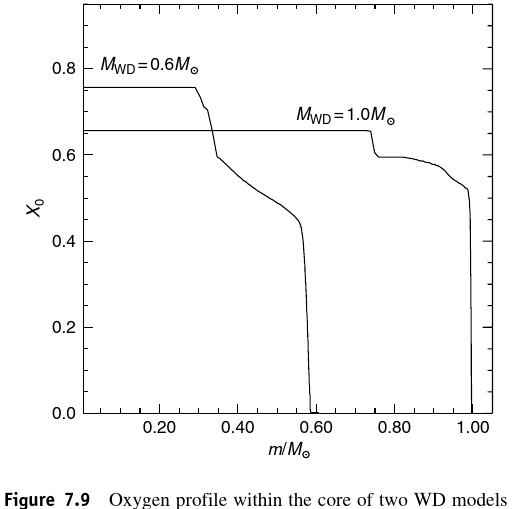
\includegraphics[trim={0cm 0cm 1cm 0cm},clip, keepaspectratio,height=0.4\textheight]{WD-Xopostcry}\label{fig:WD-Xopostcry}
		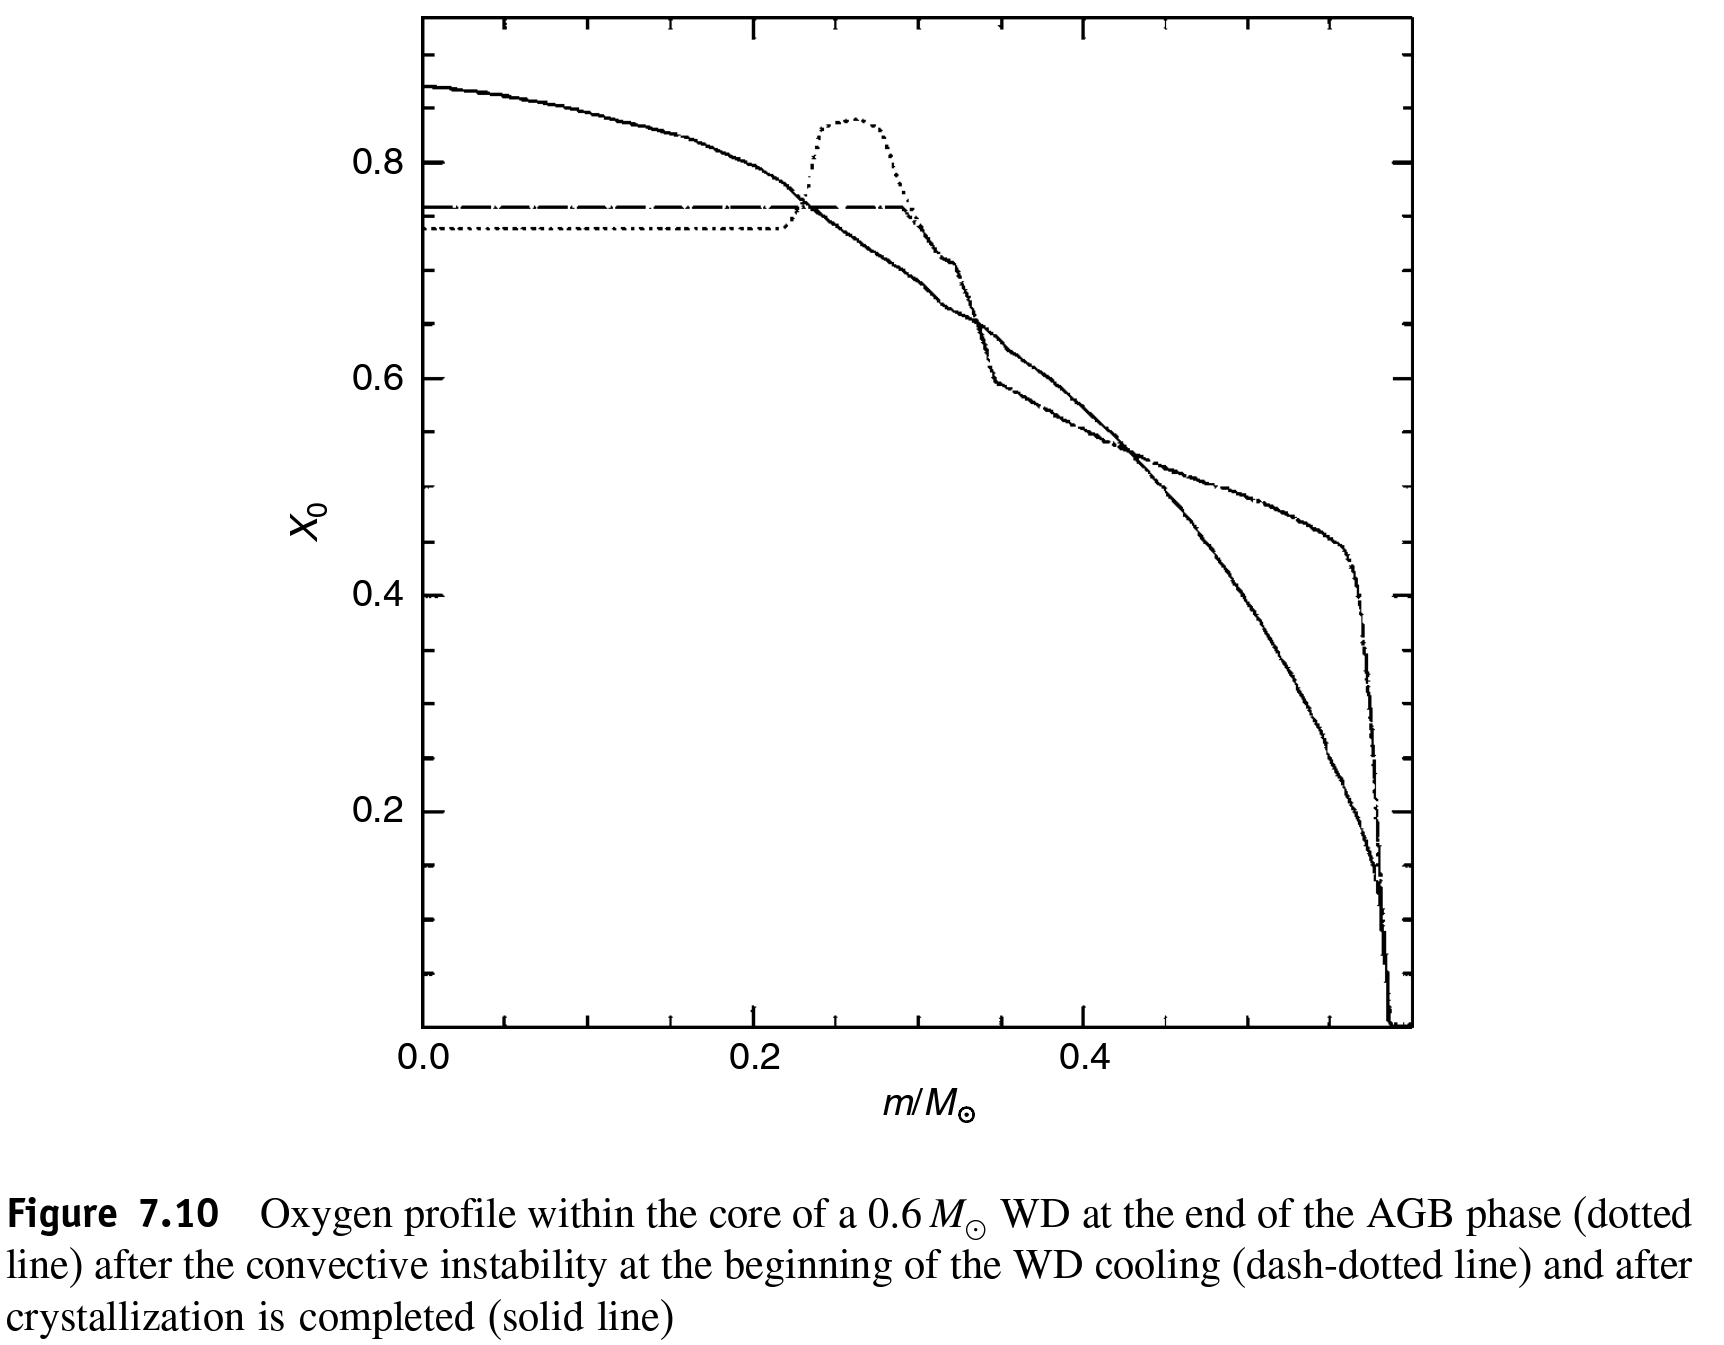
\includegraphics[trim={0cm 0cm 1cm 0cm},clip, keepaspectratio,height=0.4\textheight]{WD-AGBXo}\label{fig:WD-AGBXo}
		\end{figure}
\end{column}\end{columns}
\end{frame}

\begin{frame}{detailed computation: envelope}

		\begin{itemize}
			\item $M_{He}\approx\num{e-2}M_*$, $M_H\approx\num{e-2}M_*$, $Z_s\approx0$ - He-envelope (\keyword{Non-DA-WD}), H-envelope (\keyword{DA-WD}), $\frac{DA}{DB}\approx4$
			\item Evolution during cooling phase: intrplay between diffusion, radiative levitation and convective mixing
			\item Slow envelope contraction: $\epsilon_g$ - if $M_H>\num{e-4}\msun$, $M_{WD}\approx1\msun$ H-burning at bottom
			\item \xdiminuisce{T_e}, convective envelope (when $T_e<\SI{6000}{\kelvin}$ boundary conditions based on grey $T(\tau)$ relation no longer good approx: need full non-grey atmosphere model)
		\end{itemize}
\end{frame}


\subsection{Destino finale di stelle massicce}\linkdest{SN}

\begin{frame}{Fasi finali stelle massicce: core mass, nurning time and HDR evolution}
\begin{columns}[T]
	\begin{column}{0.65\textwidth}
		\begin{itemize}
			\item 
		\end{itemize}
	\end{column}
	\begin{column}{0.35\textwidth}
		\begin{figure}[!ht]
			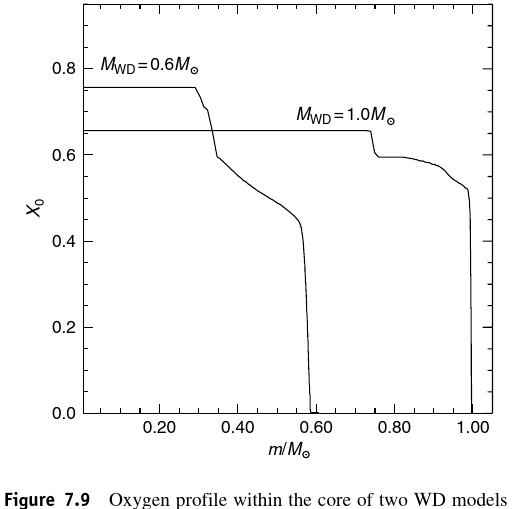
\includegraphics[trim={0cm 0cm 1cm 0cm},clip, keepaspectratio,height=0.4\textheight]{WD-Xopostcry}\label{fig:WD-Xopostcry}
			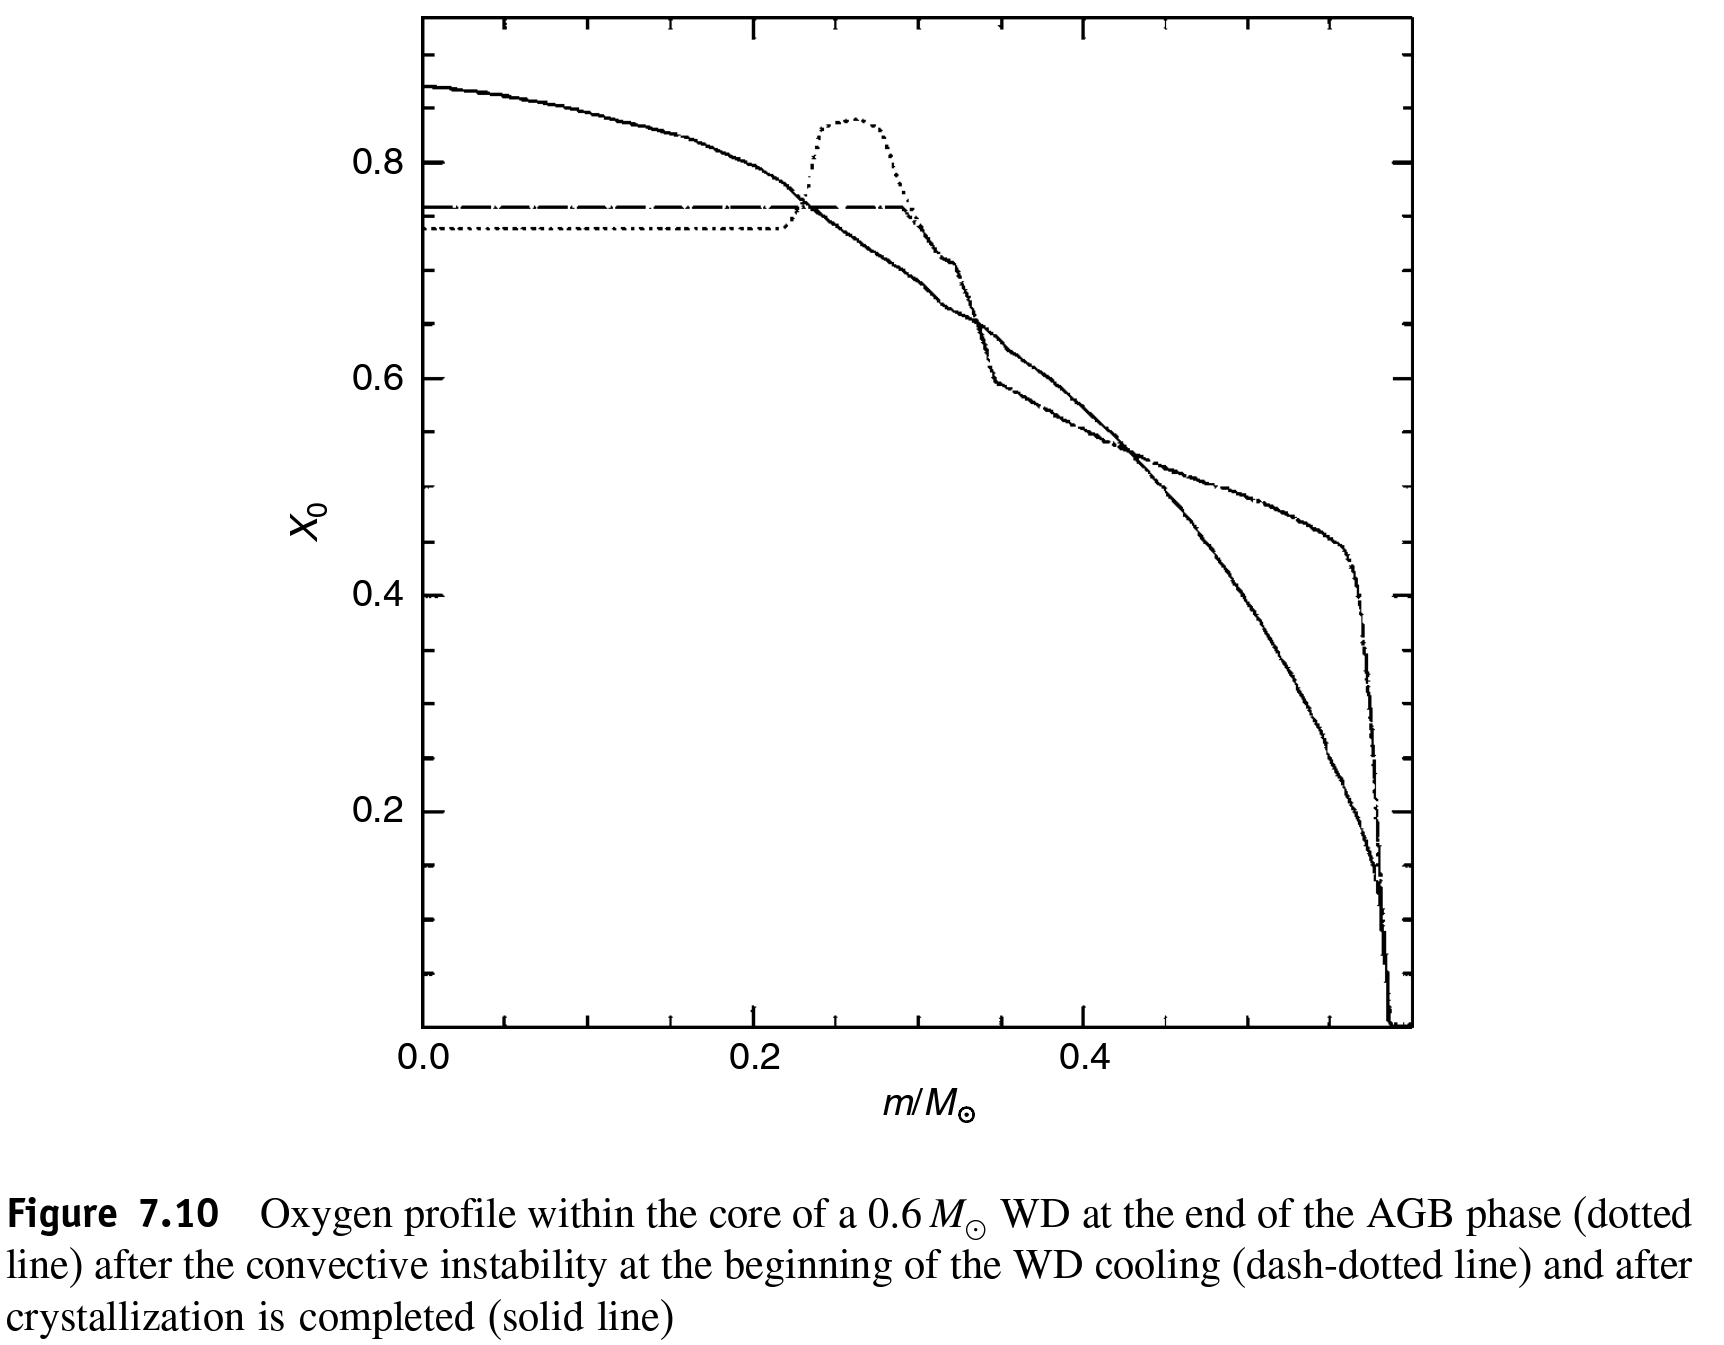
\includegraphics[trim={0cm 0cm 1cm 0cm},clip, keepaspectratio,height=0.4\textheight]{WD-AGBXo}\label{fig:WD-AGBXo}
		\end{figure}
\end{column}\end{columns}
\end{frame}


\begin{frame}{Destino finale di stelle di varia massa}
nane bianche di He, C/O, O/Ne; supernovae di tipo II da deflagrazione del carbonio e cattura elettronica su nuclei; supernovae di tipo II da fotodisintegrazione del ferro; Caratteristiche di pre-SN; Neutronizzazione esplosiva e esplosione ritardata; classificazione SN in base a spettro e morfologia curva di luce
\end{frame}



\begin{frame}{Caratterizzazione SNII}
$Fe60$ come indicatore esplosioni nelle vicinanze della terra negli ultimi milioni di anni; Interazione neutrini-nucleo denso: intrappolamento e tempi scala emissione; stima energia emessa: neutrini, fotoni, fronte di shock; SN1987A: flusso di neutrini e osservazione in bande EM
\end{frame}


\subsection{Modello Solare standar}

\begin{frame}{Caratteristiche e metodo di calcolo}
eliosismologia e neutrini
\end{frame}

\subsection{Stelle pulsanti}

\begin{frame}{Striscia di instabilit\'a e tipi di stelle pulsanti}
RR LyrAE: diagramma di Bailey, curve di luce; relazioni periodo-luminosit\'a, massa-temperatura effettiva.
Parametro A come indicatore di He.
Stelle cefeidi; dicotomia di Oosterhoff
\end{frame}